%%%%%%%%%%%%%%%%%%%%%%%%%%%%%%%%%%%%%%%%%
% Lachaise Assignment
% LaTeX Template
% Version 1.0 (26/6/2018)
%
% This template originates from:
% http://www.LaTeXTemplates.com
%
% Authors:
% Marion Lachaise & François Févotte
% Vel (vel@LaTeXTemplates.com)
%
% License:
% CC BY-NC-SA 3.0 (http://creativecommons.org/licenses/by-nc-sa/3.0/)
% 
%%%%%%%%%%%%%%%%%%%%%%%%%%%%%%%%%%%%%%%%%

%----------------------------------------------------------------------------------------
%	PACKAGES AND OTHER DOCUMENT CONFIGURATIONS
%----------------------------------------------------------------------------------------

\documentclass{article}
\usepackage{mathtools}
\usepackage{physics}
\usepackage{amsmath}
\usepackage{setspace}
\usepackage[scale=1,bmargin=1.5cm,footnotesep=1.5cm]{geometry} %footnote spacing
\usepackage{float}
\usepackage{subcaption} %allows us to nest figures

\usepackage{hyperref} %enable hyperlinks 
\hypersetup{
    colorlinks=true,
    linkcolor=violet,
    filecolor=green,      
    urlcolor=blue,
    pdftitle={Overleaf Example},
    pdfpagemode=FullScreen,
    }

% To get references:
\usepackage[nottoc,numbib]{tocbibind} % To get bibliography into table of contents
\usepackage[backend=bibtex, style=ieee]{biblatex}
\bibliography{references} 

\urlstyle{same}

%%%%%%%%%%%%%%%%%%%%%%%%%%%%%%%%%%%%%%%%%
% Lachaise Assignment
% Structure Specification File
% Version 1.0 (26/6/2018)
%
% This template originates from:
% http://www.LaTeXTemplates.com
%
% Authors:
% Marion Lachaise & François Févotte
% Vel (vel@LaTeXTemplates.com)
%
% License:
% CC BY-NC-SA 3.0 (http://creativecommons.org/licenses/by-nc-sa/3.0/)
% 
%%%%%%%%%%%%%%%%%%%%%%%%%%%%%%%%%%%%%%%%%

%----------------------------------------------------------------------------------------
%	PACKAGES AND OTHER DOCUMENT CONFIGURATIONS
%----------------------------------------------------------------------------------------

\usepackage{amsmath,amsfonts,stmaryrd,amssymb} % Math packages

\usepackage{enumerate} % Custom item numbers for enumerations

\usepackage[ruled]{algorithm2e} % Algorithms

\usepackage[framemethod=tikz]{mdframed} % Allows defining custom boxed/framed environments

\usepackage{listings} % File listings, with syntax highlighting
\lstset{
	basicstyle=\ttfamily, % Typeset listings in monospace font
}

%----------------------------------------------------------------------------------------
%	DOCUMENT MARGINS
%----------------------------------------------------------------------------------------

\usepackage{geometry} % Required for adjusting page dimensions and margins

\geometry{
	paper=a4paper, % Paper size, change to letterpaper for US letter size
	top=2.5cm, % Top margin
	bottom=3cm, % Bottom margin
	left=2.5cm, % Left margin
	right=2.5cm, % Right margin
	headheight=14pt, % Header height
	footskip=1.5cm, % Space from the bottom margin to the baseline of the footer
	headsep=1.2cm, % Space from the top margin to the baseline of the header
	%showframe, % Uncomment to show how the type block is set on the page
}

%----------------------------------------------------------------------------------------
%	FONTS
%----------------------------------------------------------------------------------------

\usepackage[utf8]{inputenc} % Required for inputting international characters
\usepackage[T1]{fontenc} % Output font encoding for international characters

\usepackage{XCharter} % Use the XCharter fonts

%----------------------------------------------------------------------------------------
%	COMMAND LINE ENVIRONMENT
%----------------------------------------------------------------------------------------

% Usage:
% \begin{commandline}
%	\begin{verbatim}
%		$ ls
%		
%		Applications	Desktop	...
%	\end{verbatim}
% \end{commandline}

\mdfdefinestyle{commandline}{
	leftmargin=10pt,
	rightmargin=10pt,
	innerleftmargin=15pt,
	middlelinecolor=black!50!white,
	middlelinewidth=2pt,
	frametitlerule=false,
	backgroundcolor=black!5!white,
	frametitle={Command Line},
	frametitlefont={\normalfont\sffamily\color{white}\hspace{-1em}},
	frametitlebackgroundcolor=black!50!white,
	nobreak,
}

% Define a custom environment for command-line snapshots
\newenvironment{commandline}{
	\medskip
	\begin{mdframed}[style=commandline]
}{
	\end{mdframed}
	\medskip
}

%----------------------------------------------------------------------------------------
%	FILE CONTENTS ENVIRONMENT
%----------------------------------------------------------------------------------------

% Usage:
% \begin{file}[optional filename, defaults to "File"]
%	File contents, for example, with a listings environment
% \end{file}

\mdfdefinestyle{file}{
	innertopmargin=1.6\baselineskip,
	innerbottommargin=0.8\baselineskip,
	topline=false, bottomline=false,
	leftline=false, rightline=false,
	leftmargin=2cm,
	rightmargin=2cm,
	singleextra={%
		\draw[fill=black!10!white](P)++(0,-1.2em)rectangle(P-|O);
		\node[anchor=north west]
		at(P-|O){\ttfamily\mdfilename};
		%
		\def\l{3em}
		\draw(O-|P)++(-\l,0)--++(\l,\l)--(P)--(P-|O)--(O)--cycle;
		\draw(O-|P)++(-\l,0)--++(0,\l)--++(\l,0);
	},
	nobreak,
}

% Define a custom environment for file contents
\newenvironment{file}[1][File]{ % Set the default filename to "File"
	\medskip
	\newcommand{\mdfilename}{#1}
	\begin{mdframed}[style=file]
}{
	\end{mdframed}
	\medskip
}

%----------------------------------------------------------------------------------------
%	NUMBERED QUESTIONS ENVIRONMENT
%----------------------------------------------------------------------------------------

% Usage:
% \begin{question}[optional title]
%	Question contents
% \end{question}

\mdfdefinestyle{question}{
	innertopmargin=1.2\baselineskip,
	innerbottommargin=0.8\baselineskip,
	roundcorner=5pt,
	nobreak,
	singleextra={%
		\draw(P-|O)node[xshift=1em,anchor=west,fill=white,draw,rounded corners=5pt]{%
		Question \theQuestion\questionTitle};
	},
}

\newcounter{Question} % Stores the current question number that gets iterated with each new question

% Define a custom environment for numbered questions
\newenvironment{question}[1][\unskip]{
	\bigskip
	\stepcounter{Question}
	\newcommand{\questionTitle}{~#1}
	\begin{mdframed}[style=question]
}{
	\end{mdframed}
	\medskip
}

%----------------------------------------------------------------------------------------
%	WARNING TEXT ENVIRONMENT
%----------------------------------------------------------------------------------------

% Usage:
% \begin{warn}[optional title, defaults to "Warning:"]
%	Contents
% \end{warn}

\mdfdefinestyle{warning}{
	topline=false, bottomline=false,
	leftline=false, rightline=false,
	nobreak,
	singleextra={%
		\draw(P-|O)++(-0.5em,0)node(tmp1){};
		\draw(P-|O)++(0.5em,0)node(tmp2){};
		\fill[black,rotate around={45:(P-|O)}](tmp1)rectangle(tmp2);
		\node at(P-|O){\color{white}\scriptsize\bf !};
		\draw[very thick](P-|O)++(0,-1em)--(O);%--(O-|P);
	}
}

% Define a custom environment for warning text
\newenvironment{warn}[1][Warning:]{ % Set the default warning to "Warning:"
	\medskip
	\begin{mdframed}[style=warning]
		\noindent{\textbf{#1}}
}{
	\end{mdframed}
}

%----------------------------------------------------------------------------------------
%	INFORMATION ENVIRONMENT
%----------------------------------------------------------------------------------------

% Usage:
% \begin{info}[optional title, defaults to "Info:"]
% 	contents
% 	\end{info}

\mdfdefinestyle{info}{%
	topline=false, bottomline=false,
	leftline=false, rightline=false,
	nobreak,
	singleextra={%
		\fill[black](P-|O)circle[radius=0.4em];
		\node at(P-|O){\color{white}\scriptsize\bf i};
		\draw[very thick](P-|O)++(0,-0.8em)--(O);%--(O-|P);
	}
}

% Define a custom environment for information
\newenvironment{info}[1][Info:]{ % Set the default title to "Info:"
	\medskip
	\begin{mdframed}[style=info]
		\noindent{\textbf{#1}}
}{
	\end{mdframed}
}
 % Include the file specifying the document structure and custom commands

%----------------------------------------------------------------------------------------

\begin{document}
\onehalfspacing
\parindent=0pt          %  Switch off indent of paragraphs

%----------------------------------------------------------------------------------------
%	TITLE PAGE
%----------------------------------------------------------------------------------------

\thispagestyle{empty}

\vspace*{0.1\textheight}

\begin{center}
        \huge{\bfseries Quantum Computing Project}\\
\end{center}

\bigskip

\begin{center}
        \large{\textbf{Group 5:}}\\
        \large{Jabeth Musumba}\\
        \large{Yi Sheng Ng}\\
        \large{Finn John Onori}\\
        \large{Tiernan Stapleton}\\
        \large{Riddhi Yadav}\\
        \large{Han Yoong}\\
        \bigskip
        \large{March 23, 2022}
\end{center}

\vspace*{0.4\textheight}

\begin{center}
        
\includegraphics[width=35mm]{crest.pdf}
\end{center}

\medskip

\newpage

%----------------------------------------------------------------------------------------
%	INTRODUCTION
%----------------------------------------------------------------------------------------
\vspace{10mm}
\hrule

\vspace{10mm}

\section*{Introduction} % Unnumbered section
\vspace{10mm}

The objective of our project is to build an application which implements the Grover's Algorithm to perform an unstructured search from a list of information.
\vspace{5mm}

\noindent
The programming language used in our project is Python. We use Git to plan, manage and organise the codes and work flow of this project. 
\vspace{5mm}

\noindent
The aim of this project is to demonstrate the basic working principle of Grover's Algorithm in the shape of a simple GUI with input and output feature.
\pagebreak

\tableofcontents % Unnumbered section
\pagebreak

\section{Introduction to Quantum Computing}
\vspace{5mm}

\subsection{Qubits}
\vspace{5mm}

The qubit can be thought of as the "quantum" counterpart to the classical bit. 
\vspace{5mm}

\noindent
A bit is expressed in binary numbers of 0 and 1. In the most simple case of a classical bit, a bit can only be in the state of 0 or 1. However as for the quantum analogue, a qubit is expressed in a superposition of both the binary state of 0 and 1.
\vspace{5mm}

\noindent
This superposition of state of a qubit $\ket{\psi}$ can be written as:
\vspace{5mm}

\begin{equation}
     \ket{\psi} = \alpha\ket{0} + \beta\ket{1}
\end{equation}
\vspace{5mm}

\noindent
Where $\alpha$ and $\beta$ are normalised complex constants such that $\abs{\alpha}^2 + \abs{\beta}^2 = 1$  for $\alpha, \ \beta \in \mathbb{C} $
\vspace{5mm}

\noindent
The quantum state of $\ket{0}$ and $\ket{1}$ are known as the computational basis state in the $\hat{\textbf{z}}$-axis on a Bloch Sphere. The basis state can be visualised in a form of a Bloch Sphere:
\vspace{5mm}

\begin{figure}[h]
  \centering
  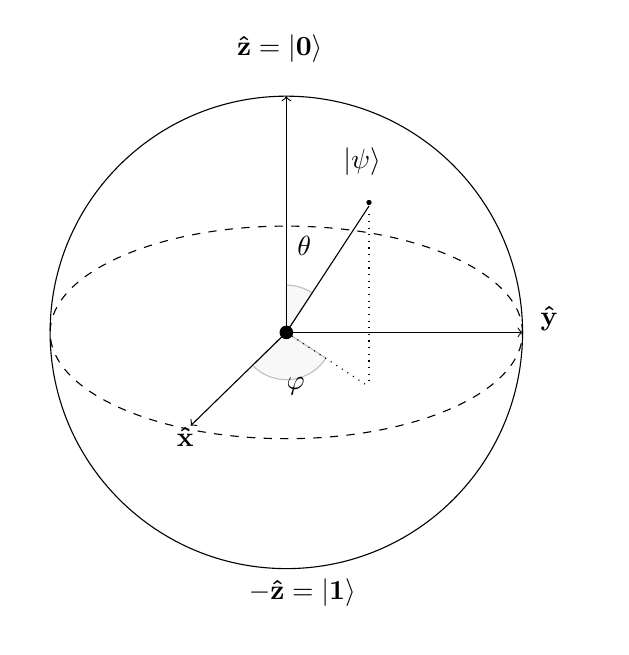
\begin{tikzpicture}[scale=1.5]
    \clip(-2.19,-2.49) rectangle (2.66,2.58);
    \draw [shift={(0,0)}, lightgray, fill, fill opacity=0.1] (0,0) -- (56.7:0.4) arc (56.7:90.:0.4) -- cycle;
    \draw [shift={(0,0)}, lightgray, fill, fill opacity=0.1] (0,0) -- (-135.7:0.4) arc (-135.7:-33.2:0.4) -- cycle;
    \draw(0,0) circle (2cm);
    \draw [rotate around={0.:(0.,0.)},dash pattern=on 3pt off 3pt] (0,0) ellipse (2cm and 0.9cm);
    \draw (0,0)-- (0.70,1.07);
    \draw [->] (0,0) -- (0,2);
    \draw [->] (0,0) -- (-0.81,-0.79);
    \draw [->] (0,0) -- (2,0);
    \draw [dotted] (0.7,1)-- (0.7,-0.46);
    \draw [dotted] (0,0)-- (0.7,-0.46);
    \draw (-0.08,-0.3) node[anchor=north west] {$\varphi$};
    \draw (0.01,0.9) node[anchor=north west] {$\theta$};
    \draw (-1.01,-0.72) node[anchor=north west] {$\mathbf {\hat{x}}$};
    \draw (2.07,0.3) node[anchor=north west] {$\mathbf {\hat{y}}$};
    \draw (-0.5,2.6) node[anchor=north west] {$\mathbf {\hat{z}=|0\rangle}$};
    \draw (-0.4,-2) node[anchor=north west] {$-\mathbf {\hat{z}=|1\rangle}$};
    \draw (0.4,1.65) node[anchor=north west] {$|\psi\rangle$};
    \scriptsize
    \draw [fill] (0,0) circle (1.5pt);
    \draw [fill] (0.7,1.1) circle (0.5pt);
  \end{tikzpicture}
  \centering
\caption{\label{fig:bloch_sphere}The Bloch Sphere}
\end{figure}
\vspace{5mm}

\noindent
These qubit states can be expressed in column matrices as:
\vspace{5mm}

\begin{equation}
\ket{0} = \begin{pmatrix}1 \\ 0 \end{pmatrix} \ \ \text{and} \ \ \ket{1} = \begin{pmatrix} 0 \\ 1 \end{pmatrix}
\end{equation}

\vspace{5mm}

\noindent
The state of a quantum system can be represented as the spin, energy, angular momentum and magnetic moment of an elementary particle. However for the sake of brevity the state $\ket{0}$ and $\ket{1}$ will denote spin up and spin down of the electron in this report.
\vspace{10mm}

\subsection{Quantum Register}
\vspace{5mm}

\noindent
The qubits in a quantum computer are stored in a quantum register. The size of the quantum register is dictated by the number of qubits. 
\vspace{5mm}

\noindent
The vector state of the quantum register $\mathcal{H}$ with $n$ qubits can be expressed in tensor product \cite{noauthor_lecture_nodate}:
\vspace{5mm}


\qquad $\mathcal{H} = \mathbb{C}^{2\bigotimes N} = \mathbb{C}^2 \bigotimes\mathbb{C}^2 ....\bigotimes\mathbb{C}^2 = \mathbb{C}^{2^N} $ , \  where the qubits are in 2-dimensional complex spaces $\mathbb{C}$.
\vspace{5mm}

\noindent
Each qubit has an index in this register, starting at index 0 and counting up by 1. So, a system with 5 qubits, for example, has a qubit register that has a width of 5 and indexed by 0, 1, 2, 3 and 4.

\subsection{Tensor Product}
\vspace{5mm}

\noindent
Tensor product is used as a function which combines elements of two or more vector spaces to yield an additional vector space. 
\vspace{5mm}

\noindent
Tensor products are distributive and associative and shown here is the tensor product of two qubits in the Hilbert space (complex vector space)\cite{noauthor_lecture_nodate}:
\vspace{5mm}


\begin{equation}
\alpha\ket{x} \bigotimes \beta\ket{y} = \alpha\beta\ket{xy}
\end{equation}
\vspace{5mm}


\begin{equation}\ket{x} \bigotimes (\ket{y} + \ket{z}) = \ket{x}\bigotimes \ket{y} + \ket{x}\bigotimes\ket{z}
\end{equation}
\vspace{5mm}


\begin{equation}
(\ket{x} + \ket{y}) \bigotimes \ket{z} = \ket{x}\bigotimes \ket{z} + \ket{y}\bigotimes\ket{z}
\end{equation}
\vspace{5mm}


\begin{equation}
(\ket{x} \bigotimes \ket{y}) \bigotimes \ket{z} = \ket{x} \bigotimes (\ket{y} \bigotimes\ket{z}) = \ket{x} \bigotimes \ket{y} \bigotimes\ket{z}
\end{equation}
\vspace{10mm}

The basis for the tensor product space is given by the product of single qubit basis states.
\vspace{5mm}

\qquad $\ket{0}_2 \bigotimes \ket{0}_1 \bigotimes \ket{0}_0 = \ket{000} = \ket{0}$
\vspace{5mm}

\qquad $\ket{0}_2 \bigotimes \ket{0}_1 \bigotimes \ket{1}_0 = \ket{001} = \ket{1}$
\vspace{5mm}

\qquad \qquad \qquad . \qquad \qquad .

\qquad \qquad \qquad . \qquad \qquad .

\qquad \qquad \qquad . \qquad \qquad .

\qquad $\ket{1}_2 \bigotimes \ket{1}_1 \bigotimes \ket{1}_0 = \ket{111} = \ket{7}$
\vspace{5mm}

Little endian notation is used to represent the qubit from right to left starting with the subscript 0.

For ease of interpretation, the binary to decimal conversion is written on the right hand side. 
\vspace{10mm}

\subsection{Linear Algebra}
\vspace{5mm}

\noindent
Linear algebra is the language of quantum computing. It is the study of vector spaces and of linear operations on vector
spaces (Hilbert space).
\vspace{5mm}

\noindent
A generic quantum state $\ket{\psi}$ can be described as a linear combination of basis states such as \cite{noauthor_lecture_nodate}:
\vspace{5mm}


\begin{equation}
\ket{\psi} = \alpha_0\ket{0} + ... + \alpha_j\ket{j} = \sum\limits_{j = 0}^{j} \alpha_j\ket{j} , \ \text{for} \alpha_j \in \mathbb{C}
\end{equation}
\vspace{5mm}

\noindent
Due to the probabilistic nature of quantum mechanics, the state must be normalised, i.e $\sum\limits_j |\alpha_j|^2 = 1$
\vspace{5mm}

\noindent
The action of quantum operators on a state is linear. For a quantum operator $U$ acting on some state $\{\ket{x}$ and $\ket{y}$ can be expressed as:
\vspace{5mm}

\noindent
\begin{equation}
U(\alpha\ket{x} + \beta\ket{y}) = \alpha U\ket{x} + \beta U\ket{x} , \ \text{for} \alpha, \beta \in \mathbb{C}
\end{equation}
\vspace{5mm}

\noindent
The action of a quantum linear operator on a basis state determines the type of operator it is. It can also act on multiple or superposition of basis states:
\vspace{5mm}

\noindent
\begin{equation}
U \sum\limits_j \alpha_j \ket{j} = \sum\limits_j \alpha_j U\ket{j}
\end{equation}
\vspace{10mm}

\subsection{Matrix Operation}
\vspace{5mm}

\noindent
Linear operators $U$ acting on some basis states can be written in matrix form \cite{noauthor_lecture_nodate}:
\vspace{5mm}

\begin{equation}
U_{kj} = \bra{k}U\ket{j} \ , \text{for some basis state} \ket{j} \text{and} \ket{k} 
\end{equation}
\vspace{5mm}

\noindent
By using the Completeness Relation of quantum mechanics:
\vspace{5mm}

\begin{equation}
U\ket{j} = \underbrace{\sum\limits_k\ket{k}\bra{k}}_{ = 1} U\ket{j} = \sum\limits_k \ket{k} U_{kj}    
\end{equation}
\vspace{5mm}

\noindent
Multiple linear operators applied on a basis state can be written as:
\vspace{5mm}

\begin{equation}
UV\ket{k} = U\sum\limits_k \ket{k}V_{kj} = \sum\limits_l\ket{l} \sum\limits_k U_{lk} V_{kj} = \sum\limits_l(UV)_{lj}
\end{equation}
\vspace{5mm}

\noindent
The linear operator $U$ acting on the coefficient $\alpha$ of the vector state $\ket{\psi}$ can be expressed:
\vspace{5mm}

\begin{equation}
\alpha' = U\alpha
\end{equation}
\vspace{5mm}

\noindent
And on the state:
\vspace{5mm}

\begin{equation}
ket{\psi'} = U\ket{\psi}
\end{equation}
\vspace{5mm}

\noindent
Additionally, all quantum operators (quantum gates) are unitary with the exception of measurement and reset operators. 
\vspace{5mm}

\noindent
A quantum operator $U$ has its conjugate transpose (adjoint) which can be expressed as $U^{\dagger}$.
\vspace{5mm}

\noindent
The unitary operator has the following property\cite{noauthor_unitary_2022}:
\vspace{5mm}

\begin{equation}
UU^{\dagger} = UU^{-1} = 1    
\end{equation}
\vspace{5mm}

\noindent
Another consequence of unitarity is that it preserves the inner product between two arbitrary states $\braket{\phi}{\psi}$. For example apply the unitary operator $U$ to two states $\ket{\phi}$ and $\ket{\psi}$:
\vspace{5mm}

\begin{equation}
\bra{\phi} U^{\dagger} U\ket{\psi} = \braket{\phi}{\psi}
\end{equation}
\vspace{5mm}

\noindent
the inner product of the resulting states is exactly the same,
\vspace{10mm}


\subsection{Gates and Operators}
\vspace{5mm}

Quantum gates are unitary quantum operators and are described as unitary matrices relative to some basis states.
\vspace{5mm}

\noindent
The following are some of the common types of quantum gates\cite{voorhoede_pauli-x_nodate} which will be used in constructing the Grover's circuit.
\vspace{5mm}

\textbf{Hadamard Gate}: \qquad $H = \frac{1}{\sqrt{2}} \begin{pmatrix} 1 & 1 \\ 1 & -1 \end{pmatrix}$
\vspace{5mm}

\noindent
The Hadamard gate creates a superposition states when acted on a state:
\vspace{5mm}


\begin{equation}
H\ket{0} = \frac{1}{\sqrt{2}} (\ket{0} + \ket{1}), \ \ H\ket{1} = \frac{1}{\sqrt{2}}(\ket{0} - \ket{1})   
\end{equation}
\vspace{5mm}

\noindent
This can then be generalised as:
\vspace{5mm}

\begin{equation}
H\ket{j} = \frac{-1^j\ket{j} + \ket{1 - j}}{\sqrt{2}} 
\end{equation}
\vspace{5mm}


\textbf{Pauli X Gate}: \qquad $X = \begin{pmatrix} 0 & 1 \\ 1 & 0 \end{pmatrix}$
\vspace{5mm}


\begin{equation}
X\ket{0} = \ket{1} , \ \ X\ket{1} = \ket{0}
\end{equation}
\vspace{5mm}

\noindent
The Pauli X Gate essentially swaps the qubits around. This effect of this gate is also known as bit flip. The gate is a single qubit rotation around the x-axis by $\pi$
\vspace{5mm}


\textbf{Pauli Y Gate}: \qquad $Y = \begin{pmatrix} 0 & -i \\ i & 0 \end{pmatrix}$
\vspace{5mm}


\begin{equation}
Y\ket{0} = i\ket{1} , \ \ Y\ket{1} = -i\ket{0}
\end{equation}
\vspace{5mm}

\noindent
The Pauli Y Gate rotates a single qubit in the y (complex)-axis by $\pi$.
\vspace{5mm}


\textbf{Pauli Z Gate}: \qquad $Z = \begin{pmatrix} 1 & 0 \\ 0 & -1 \end{pmatrix}$
\vspace{5mm}


\begin{equation}
Z\ket{0} = \ket{0} , \ \ Z\ket{1} = -\ket{1}  
\end{equation}
\vspace{5mm}

\noindent
The Pauli-Z gate is a single qubit rotation through $\pi$ radians around the z-axis. The effect of the Pauli Z Gate is also known as phase-flip.
\vspace{5mm}

\textbf{Controlled Not/CNOT Gate}: \qquad CNOT = $\begin{pmatrix} 1 & 0 & 0 & 0 \\ 0 & 1 & 0 & 0 \\ 0 & 0 & 0 & 1 \\ 0 & 0 & 1 & 0 \end{pmatrix}$
\vspace{5mm}

\noindent
The CNOT Gate is a two qubit gate which takes the first qubit as the control qubit and the second qubit as the target qubit.
\vspace{5mm}

\noindent
It leaves the control qubit unchanged and performs the Pauli X Gate to the target qubit if and only if when the control qubit is $\ket{1}$ and leaves the target qubit unchanged when the control qubit is $\ket{0}$.
\vspace{5mm}

\textbf{Controlled Z/CZ Gate}: \qquad CZ = $\begin{pmatrix} 1 & 0 & 0 & 0 \\ 0 & 1 & 0 & 0 \\ 0 & 0 & 1 & 0 \\ 0 & 0 & 0 & -1 \end{pmatrix}$
\vspace{5mm}

\noindent
The CZ Gate is a two qubit gate which takes the first qubit as the control qubit and the second qubit as the target qubit.
\vspace{5mm}

\noindent
It leaves the control qubit unchanged and performs the Pauli Z Gate to the target qubit if and only if when the control qubit is $\ket{1}$ and leaves the target qubit unchanged when the control qubit is $\ket{0}$.
\pagebreak

\textbf{Phase Shift Gates}: \qquad $ P(\varphi) = \begin{pmatrix} 1 & 0 \\ 0 & e^{i\varphi} \end{pmatrix}$ 
\vspace{5mm}

\begin{equation}
P(\varphi)\ket{0} = \ket{0} \ \text{and} \ P(\varphi)\ket{1} = e^{i\varphi}\ket{1} 
\end{equation}

\noindent
The phase shift gate modifies the phase of the quantum state and is equivalent to tracing a horizontal circle on the Bloch Sphere (see Figure \ref{fig:bloch_sphere}) by $\varphi$ radians\cite{noauthor_quantum_nodate}. 
\pagebreak






\section{Grover's Algorithm}
\subsection{Introduction}

The Grover's Algorithm is a quantum search algorithm which increases quadratically the speed of unstructured search\cite{noauthor_grovers_nodate}. It uses  amplitude amplification to search an unstructured set of $N$ elements/items. 

\subsection{Unstructured Search}
\vspace{10mm}

\begin{figure}[h]
  \begin{center}

    \tikzset{every picture/.style={line width=0.75pt}} %set default line width to 0.75pt        

    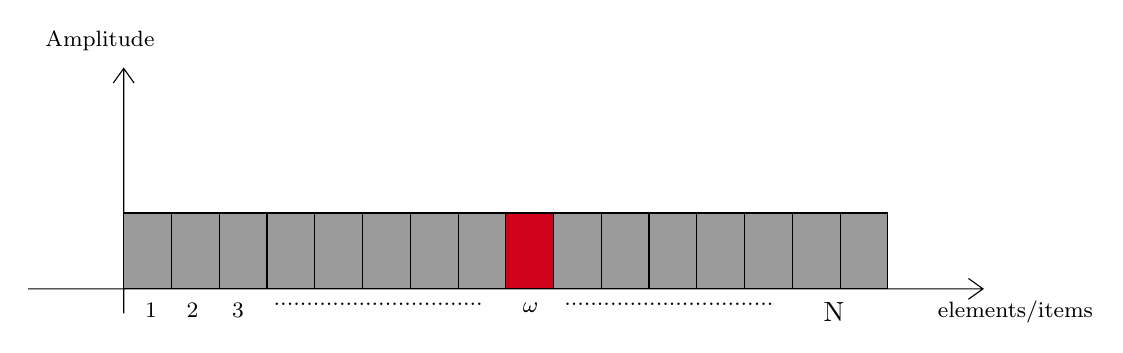
\begin{tikzpicture}[x=0.75pt,y=0.75pt,yscale=-1,xscale=1]
      %uncomment if require: \path (0,310); %set diagram left start at 0, and has height of 310

      %Shape: Axis 2D [id:dp7326811016330554] 
      \draw  (54,256.57) -- (514,256.57)(100,150.37) -- (100,268.37) (507,251.57) -- (514,256.57) -- (507,261.57) (95,157.37) -- (100,150.37) -- (105,157.37)  ;
      %Shape: Rectangle [id:dp9165080769461678] 
      \draw  [fill={rgb, 255:red, 155; green, 155; blue, 155 }  ,fill opacity=1 ] (100,220) -- (123.02,220) -- (123.02,256.57) -- (100,256.57) -- cycle ;
      %Shape: Rectangle [id:dp6197087457024866] 
      \draw  [fill={rgb, 255:red, 155; green, 155; blue, 155 }  ,fill opacity=1 ] (123.02,220) -- (146.04,220) -- (146.04,256.57) -- (123.02,256.57) -- cycle ;
      %Shape: Rectangle [id:dp5818508515663341] 
      \draw  [fill={rgb, 255:red, 155; green, 155; blue, 155 }  ,fill opacity=1 ] (146.04,220) -- (169.06,220) -- (169.06,256.57) -- (146.04,256.57) -- cycle ;
      %Shape: Rectangle [id:dp6466988498042014] 
      \draw  [fill={rgb, 255:red, 155; green, 155; blue, 155 }  ,fill opacity=1 ] (169.06,220) -- (192.08,220) -- (192.08,256.57) -- (169.06,256.57) -- cycle ;
      %Shape: Rectangle [id:dp9241747490680354] 
      \draw  [fill={rgb, 255:red, 155; green, 155; blue, 155 }  ,fill opacity=1 ] (192.08,220) -- (215.1,220) -- (215.1,256.57) -- (192.08,256.57) -- cycle ;
      %Shape: Rectangle [id:dp6900943731279547] 
      \draw  [fill={rgb, 255:red, 155; green, 155; blue, 155 }  ,fill opacity=1 ] (215.1,220) -- (238.12,220) -- (238.12,256.57) -- (215.1,256.57) -- cycle ;
      %Shape: Rectangle [id:dp9784662305616809] 
      \draw  [fill={rgb, 255:red, 155; green, 155; blue, 155 }  ,fill opacity=1 ] (238.12,220) -- (261.14,220) -- (261.14,256.57) -- (238.12,256.57) -- cycle ;
      %Shape: Rectangle [id:dp3189854749942387] 
      \draw  [fill={rgb, 255:red, 155; green, 155; blue, 155 }  ,fill opacity=1 ] (261.14,220) -- (284.16,220) -- (284.16,256.57) -- (261.14,256.57) -- cycle ;
      %Shape: Rectangle [id:dp19644432939638312] 
      \draw  [fill={rgb, 255:red, 208; green, 2; blue, 27 }  ,fill opacity=1 ] (284.04,220) -- (307.06,220) -- (307.06,256.57) -- (284.04,256.57) -- cycle ;
      %Shape: Rectangle [id:dp4454731461786199] 
      \draw  [fill={rgb, 255:red, 155; green, 155; blue, 155 }  ,fill opacity=1 ] (307.06,220) -- (330.08,220) -- (330.08,256.57) -- (307.06,256.57) -- cycle ;
      %Shape: Rectangle [id:dp8963311487850567] 
      \draw  [fill={rgb, 255:red, 155; green, 155; blue, 155 }  ,fill opacity=1 ] (330.08,220) -- (353.1,220) -- (353.1,256.57) -- (330.08,256.57) -- cycle ;
      %Shape: Rectangle [id:dp8621164913285171] 
      \draw  [fill={rgb, 255:red, 155; green, 155; blue, 155 }  ,fill opacity=1 ] (353.1,220) -- (376.12,220) -- (376.12,256.57) -- (353.1,256.57) -- cycle ;
      %Shape: Rectangle [id:dp7667099225825136] 
      \draw  [fill={rgb, 255:red, 155; green, 155; blue, 155 }  ,fill opacity=1 ] (376.12,220) -- (399.14,220) -- (399.14,256.57) -- (376.12,256.57) -- cycle ;
      %Shape: Rectangle [id:dp1405504024872024] 
      \draw  [fill={rgb, 255:red, 155; green, 155; blue, 155 }  ,fill opacity=1 ] (399.14,220) -- (422.16,220) -- (422.16,256.57) -- (399.14,256.57) -- cycle ;
      %Shape: Rectangle [id:dp6549374163542783] 
      \draw  [fill={rgb, 255:red, 155; green, 155; blue, 155 }  ,fill opacity=1 ] (422.16,220) -- (445.18,220) -- (445.18,256.57) -- (422.16,256.57) -- cycle ;
      %Shape: Rectangle [id:dp26369533307147797] 
      \draw  [fill={rgb, 255:red, 155; green, 155; blue, 155 }  ,fill opacity=1 ] (445.18,220) -- (468.2,220) -- (468.2,256.57) -- (445.18,256.57) -- cycle ;

      % Text Node
      \draw (491,261) node [anchor=north west][inner sep=0.75pt]   [align=left] {{\footnotesize elements/items}};
      % Text Node
      \draw (61,131) node [anchor=north west][inner sep=0.75pt]   [align=left] {{\footnotesize Amplitude}};
      % Text Node
      \draw (109,262) node [anchor=north west][inner sep=0.75pt]  [font=\footnotesize] [align=left] {1};
      % Text Node
      \draw (129,262) node [anchor=north west][inner sep=0.75pt]  [font=\footnotesize] [align=left] {2};
      % Text Node
      \draw (171,262) node [anchor=north west][inner sep=0.75pt]  [font=\footnotesize] [align=left] {................................};
      % Text Node
      \draw (151,262) node [anchor=north west][inner sep=0.75pt]  [font=\footnotesize] [align=left] {3};
      % Text Node
      \draw (311,262) node [anchor=north west][inner sep=0.75pt]  [font=\footnotesize] [align=left] {................................};
      % Text Node
      \draw (291,262) node [anchor=north west][inner sep=0.75pt]  [font=\footnotesize] [align=left] {$\displaystyle \omega $};
      % Text Node
      \draw (436,262) node [anchor=north west][inner sep=0.75pt]   [align=left] {N};

    \end{tikzpicture}    
  \end{center}
  \caption{\label{fig:intial_quantum_state} The initial quantum state}
\end{figure}

\vspace{10mm}
\noindent
An unstructured search through a list of items using Grover's Algorithm can be illustrated in Figure1. In this instance, $\omega$ the red block, represents the item which we want to find and $N$ represents the number of items in the list. 
\vspace{5mm}

\noindent
On classical computation, $\omega$ must check at least on average $O(N/2)$ entries of the list which gives $\frac{1}{2}$ the probability of finding $\omega$ or worse the entire N elements in the list.
With Grover's Algorithm, only $O(\sqrt{N})$ steps are required to find $\omega$.
\vspace{5mm}

\noindent
For an $N$ item search problem with $M$ number of solutions, the required number of times of searches will be $O(\sqrt{\frac{N}{M}})$\cite{nielsen_quantum_2010}.
\pagebreak

\subsection{The Oracle}
\vspace{5mm}

Let's suppose the function $f$ of $N$ integer such that $f:\{0,1, 2,...., N-1\} \rightarrow{\{0,1\}}$. 
\vspace{5mm}

\noindent
The integers in the domain corresponds to the indices of the list and $f(x) =1$ if and only if $x$ corresponds to the item which is searched conversely $f(x) =0$ for $x$ not corresponding the item searched. 
\vspace{5mm}

\noindent
There will be only one value of $x$ which satisfies $f(x)=1$ and this index corresponds to item $\omega$\cite{noauthor_grovers_2022}.
\vspace{5mm}

\noindent
So $f$ can be accessed with a unitary operator $U_{\omega}$ of  an oracle which satisfies:
\vspace{5mm}

\begin{equation}
\begin{cases}
      U_{\omega}\ket{x} = -\ket{x}  & \text{for} \ x = \omega, \ f(x) =1 \\
       U_{\omega}\ket{x} = \ket{x}  & \text{for} \ x \neq \omega, \ f(x) = 0 \\
\end{cases}  
\end{equation}

\vspace{5mm}

The oracle function of a two qubit system is defined as\cite{j_quantum_2020}:
\vspace{5mm}

\begin{equation}
\ket{x} \bigotimes \ket{q} \rightarrow{O_f} \ket{x} \bigotimes \ket{q \bigoplus f(x)} \footnote{$\bigotimes$ denotes tensor product and $\bigoplus$ denotes denotes addition modulo 2}  
\end{equation}

\vspace{5mm}

\begin{equation}
\ket{q} = \frac{\ket{0} - \ket{1}}{\sqrt{2}}
\end{equation}
\vspace{5mm}

Substitute $\ket{q}$ into the oracle function $O_f$:
\vspace{5mm}

\begin{equation}
 O\ket{x}\frac{\ket{0} - \ket{1}}{\sqrt{2}} \rightarrow \ket{x} \frac{\ket{f(x) \bigoplus 0} - \ket{f(x) \bigoplus 1}}{\sqrt{2}}    
\end{equation}
\vspace{5mm}

\begin{equation}
\text{if} \ f(x) =1 \rightarrow \ket{x}\frac{\ket{f(x) \bigoplus0} - \ket{f(x) \bigoplus1}}{\sqrt{2}}   
\end{equation}
\vspace{5mm}

\begin{equation}
\text{if} \ f(x) =1 \rightarrow \ket{x}\frac{\ket{1 \bigoplus 0} - \ket{1 \bigoplus 1}}{\sqrt{2}} = -\ket{x}\frac{\ket{0} - \ket{1}}{\sqrt{2}}    
\end{equation}
\vspace{5mm}

\begin{equation}
\text{if} \ f(x) =0 \rightarrow \ket{x}\frac{\ket{0 \bigoplus 0} - \ket{0 \bigoplus 1}}{\sqrt{2}} = \ket{x}\frac{\ket{0} - \ket{1}}{\sqrt{2}}    
\end{equation}
\vspace{5mm}

\noindent
When $f(x) = 1 $, the amplitude $\ket{x}$ changed to negative and remains unchanged when $f(x) = 0$.
\vspace{5mm}

\noindent
The oracle takes the form of a diagonal matrix $U_{\omega}$
\vspace{5mm}
\noindent
For example, in a three qubit state, we want to look for the number 6 which corresponds to $\ket{110}$. In matrix form $\omega =6$ will be:
\vspace{5mm}

\qquad $ U_\omega = \begin{bmatrix}

1 & 0 & 0 & 0 & 0& 0 & 0& 0 \\
0 & 1 & 0 & 0 & 0& 0 & 0& 0 \\
0 & 0 & 1 & 0 & 0& 0 & 0& 0 \\
0 & 0 & 0 & 1 & 0& 0 & 0& 0 \\
0 & 0 & 0 & 0 & 1& 0 & 0& 0 \\
0 & 0 & 0 & 0 & 0& 1 & 0& 0 \\
0 & 0 & 0 & 0 & 0& 0 & -1& 0 \\
0 & 0 & 0 & 0 & 0& 0 & 0& 1 \\

\end{bmatrix}$
\vspace{5mm}

Hence the oracle can be described as:
\vspace{5mm}

\begin{equation}
U_\omega\ket{x} = (-1)^{f(x)} \ket{x}    
\end{equation}
\vspace{5mm}

This is essentially a reflection on the state $\ket{x}$.

\pagebreak

\subsection{How The Algorithm Works}
\vspace{5mm}

\textbf{Step 1:}
\vspace{5mm}
\noindent
The sequence of the Grover's Algorithm starts out with a uniform superposition state $\ket{s}$\cite{noauthor_grovers_nodate}:
\vspace{5mm}

\begin{equation}
\ket{s}= H^{\bigotimes n} \ket{0}^n = \frac{1}{\sqrt{2^n}}\sum\limits_{x \in \{0,1\}^n}\ket{x}
\end{equation}
\vspace{5mm}

\qquad For $N = 2^n$ , where $n$ is the number of qubits.
\vspace{5mm}


\begin{figure}[h]
  \begin{subfigure}{.5\textwidth}
    \centering
    \tikzset{every picture/.style={line width=0.75pt}} %set default line width to 0.75pt

    \begin{tikzpicture}[x=0.75pt,y=0.75pt,yscale=-1,xscale=1]
      % uncomment if require: \path (0,300); %set diagram left start at 0, and has height of 300

      %Shape: Axis 2D [id:dp05560542711234939] 
      \draw  (50,247.9) -- (308,247.9)(75.8,112) -- (75.8,263) (301,242.9) -- (308,247.9) -- (301,252.9) (70.8,119) -- (75.8,112) -- (80.8,119)  ;
      %Shape: Boxed Line [id:dp13553556978051007] 
      \draw    (75.8,247.9) -- (298.07,185.84) ;
      \draw [shift={(300,185.3)}, rotate = 164.4] [color={rgb, 255:red, 0; green, 0; blue, 0 }  ][line width=0.75]    (10.93,-3.29) .. controls (6.95,-1.4) and (3.31,-0.3) .. (0,0) .. controls (3.31,0.3) and (6.95,1.4) .. (10.93,3.29)   ;

      % Text Node
      \draw (82,87.4) node [anchor=north west][inner sep=0.75pt]    {$\ket{\omega }$};
      % Text Node
      \draw (306,167.4) node [anchor=north west][inner sep=0.75pt]    {$\ket{s}$};
      % Text Node
      \draw (307,253.4) node [anchor=north west][inner sep=0.75pt]    {$\ket{s'}$};
      % Text Node
      \draw (181,220.4) node [anchor=north west][inner sep=0.75pt]    {$\theta $};

    \end{tikzpicture}

    \caption{\label{fig:grover_step_1a} Grover's Algorithm Step 1a}
  \end{subfigure}%
  \begin{subfigure}{.5\textwidth}
    \centering
    \tikzset{every picture/.style={line width=0.75pt}} %set default line width to 0.75pt        

    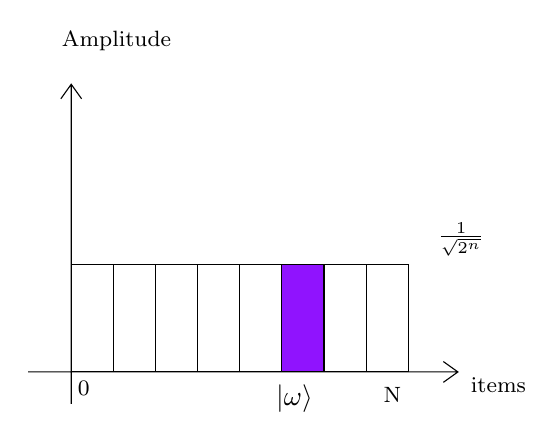
\begin{tikzpicture}[x=0.75pt,y=0.75pt,yscale=-1,xscale=1]
      %uncomment if require: \path (0,300); %set diagram left start at 0, and has height of 300

      %Shape: Axis 2D [id:dp29246180096889995] 
      \draw  (390,249.6) -- (597,249.6)(410.7,111) -- (410.7,265) (590,244.6) -- (597,249.6) -- (590,254.6) (405.7,118) -- (410.7,111) -- (415.7,118)  ;
      %Shape: Rectangle [id:dp09588343067912675] 
      \draw   (410.7,198) -- (431,198) -- (431,249.6) -- (410.7,249.6) -- cycle ;
      %Shape: Rectangle [id:dp06589745305688277] 
      \draw   (431,198) -- (451.3,198) -- (451.3,249.6) -- (431,249.6) -- cycle ;
      %Shape: Rectangle [id:dp1570793013008731] 
      \draw   (451.3,198) -- (471.6,198) -- (471.6,249.6) -- (451.3,249.6) -- cycle ;
      %Shape: Rectangle [id:dp04465276081897107] 
      \draw   (471.6,198) -- (491.9,198) -- (491.9,249.6) -- (471.6,249.6) -- cycle ;
      %Shape: Rectangle [id:dp3205832207723005] 
      \draw   (491.9,198) -- (512.2,198) -- (512.2,249.6) -- (491.9,249.6) -- cycle ;
      %Shape: Rectangle [id:dp7965850817244042] 
      \draw  [fill={rgb, 255:red, 144; green, 19; blue, 254 }  ,fill opacity=1 ] (512.2,198) -- (532.5,198) -- (532.5,249.6) -- (512.2,249.6) -- cycle ;
      %Shape: Rectangle [id:dp41205715411636223] 
      \draw   (532.5,198) -- (552.8,198) -- (552.8,249.6) -- (532.5,249.6) -- cycle ;
      %Shape: Rectangle [id:dp6260805143227606] 
      \draw   (552.8,198) -- (573.1,198) -- (573.1,249.6) -- (552.8,249.6) -- cycle ;

      % Text Node
      \draw (405,84) node [anchor=north west][inner sep=0.75pt]   [align=left] {{\footnotesize Amplitude}};
      % Text Node
      \draw (412.7,252.6) node [anchor=north west][inner sep=0.75pt]   [align=left] {{\footnotesize 0}};
      % Text Node
      \draw (586,176.4) node [anchor=north west][inner sep=0.75pt]  [font=\footnotesize]  {$\frac{1}{\sqrt{2^{n}}}$};
      % Text Node
      \draw (560,256) node [anchor=north west][inner sep=0.75pt]   [align=left] {{\footnotesize N}};
      % Text Node
      \draw (602,251) node [anchor=north west][inner sep=0.75pt]   [align=left] {{\footnotesize items}};
      % Text Node
      \draw (508.2,254.4) node [anchor=north west][inner sep=0.75pt]    {$\ket{\omega }$};

    \end{tikzpicture}
    \caption{\label{fig:grover_step_1b} Grover's Algorithm Step 1b}
  \end{subfigure}
  \caption{\label{fig:grover_step_1} Grover's Algorithm Step 1}
\end{figure}
\vspace{5mm}

Figure \ref{fig:grover_step_1a} shows a two dimensional plane spanned by $\ket{\omega}$ and $\ket{s'}$. In this representation, it can be written:
\vspace{5mm}

\begin{equation}
\ket{s} = \sin\theta\ket{\omega} + \cos\theta\ket{s'}   
\end{equation}
\vspace{5mm}

\begin{equation}
\sin\theta = \frac{1}{\sqrt{2^n}}    
\end{equation}
\vspace{5mm}

Where the amplitude of $\ket{s}$ is as shown in Figure \ref{fig:grover_step_1b}.
\pagebreak

\textbf{Step 2:}
\vspace{5mm}
Next apply the reflection oracle $U_\omega$ to the state $\ket{s}$.
\vspace{5mm}


\begin{figure}[h]
  \begin{subfigure}{0.5\textwidth}
    \centering
    \tikzset{every picture/.style={line width=0.75pt}} %set default line width to 0.75pt        
    
    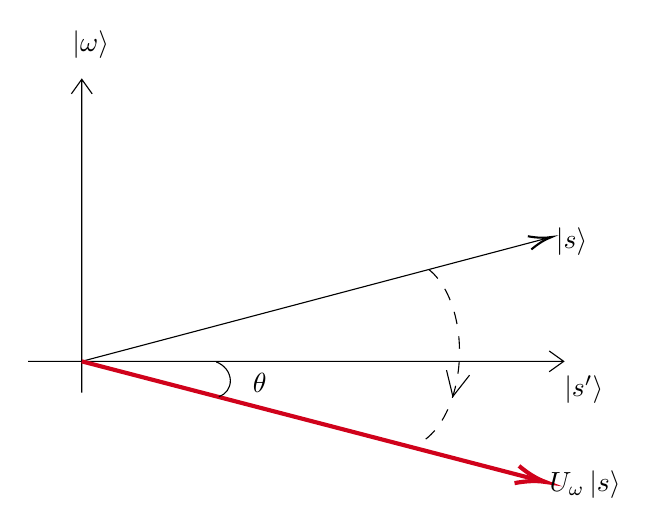
\begin{tikzpicture}[x=0.75pt,y=0.75pt,yscale=-1,xscale=1]
        %uncomment if require: \path (0,421); %set diagram left start at 0, and has height of 421
        
        %Shape: Axis 2D [id:dp9468133521588677] 
        \draw  (50,250.9) -- (308,250.9)(75.8,115) -- (75.8,266) (301,245.9) -- (308,250.9) -- (301,255.9) (70.8,122) -- (75.8,115) -- (80.8,122)  ;
        %Shape: Boxed Line [id:dp05857323871196929] 
        \draw    (75.8,250.9) -- (300.2,191.51) ;
        \draw [shift={(302.13,191)}, rotate = 165.18] [color={rgb, 255:red, 0; green, 0; blue, 0 }  ][line width=0.75]    (10.93,-3.29) .. controls (6.95,-1.4) and (3.31,-0.3) .. (0,0) .. controls (3.31,0.3) and (6.95,1.4) .. (10.93,3.29)   ;
        %Shape: Boxed Line [id:dp6041685570388957] 
        \draw [color={rgb, 255:red, 208; green, 2; blue, 27 }  ,draw opacity=1 ][fill={rgb, 255:red, 74; green, 144; blue, 226 }  ,fill opacity=1 ][line width=1.5]    (75.8,250.9) -- (296.23,308.24) ;
        \draw [shift={(299.13,309)}, rotate = 194.58] [color={rgb, 255:red, 208; green, 2; blue, 27 }  ,draw opacity=1 ][line width=1.5]    (14.21,-4.28) .. controls (9.04,-1.82) and (4.3,-0.39) .. (0,0) .. controls (4.3,0.39) and (9.04,1.82) .. (14.21,4.28)   ;
        %Shape: Arc [id:dp7847818797073434] 
        \draw  [draw opacity=0][dash pattern={on 4.5pt off 4.5pt}] (243.13,206.74) .. controls (255.6,216.75) and (261.2,241.7) .. (255.64,263.91) .. controls (252.12,278.01) and (244.9,287.75) .. (236.73,291.16) -- (231.03,247.47) -- cycle ; \draw  [dash pattern={on 4.5pt off 4.5pt}] (243.13,206.74) .. controls (255.6,216.75) and (261.2,241.7) .. (255.64,263.91) .. controls (252.12,278.01) and (244.9,287.75) .. (236.73,291.16) ;  
        \draw   (262.62,257.57) -- (254.59,267.79) -- (251.53,255.15) ;
        %Shape: Arc [id:dp2964811498005937] 
        \draw  [draw opacity=0] (140.64,251.2) .. controls (144.47,252.64) and (147.27,256.11) .. (147.38,260.04) .. controls (147.48,263.72) and (145.19,266.77) .. (141.81,268.01) -- (137.59,259.56) -- cycle ; \draw   (140.64,251.2) .. controls (144.47,252.64) and (147.27,256.11) .. (147.38,260.04) .. controls (147.48,263.72) and (145.19,266.77) .. (141.81,268.01) ;  
        
        % Text Node
        \draw (70,90.4) node [anchor=north west][inner sep=0.75pt]    {$\ket{\omega }$};
        % Text Node
        \draw (303,185.4) node [anchor=north west][inner sep=0.75pt]    {$\ket{s}$};
        % Text Node
        \draw (307,256.4) node [anchor=north west][inner sep=0.75pt]    {$\ket{s'}$};
        % Text Node
        \draw (157,255.4) node [anchor=north west][inner sep=0.75pt]    {$\theta $};
        % Text Node
        \draw (300,302.4) node [anchor=north west][inner sep=0.75pt]    {$U_{\omega }\ket{s}$};
    \end{tikzpicture}
    
    \caption{\label{fig:grover_step_2a} Grover's Algorithm Step 2a}
  \end{subfigure}%
  \begin{subfigure}{0.5\textwidth}
      \centering
      \tikzset{every picture/.style={line width=0.75pt}} %set default line width to 0.75pt        
      
      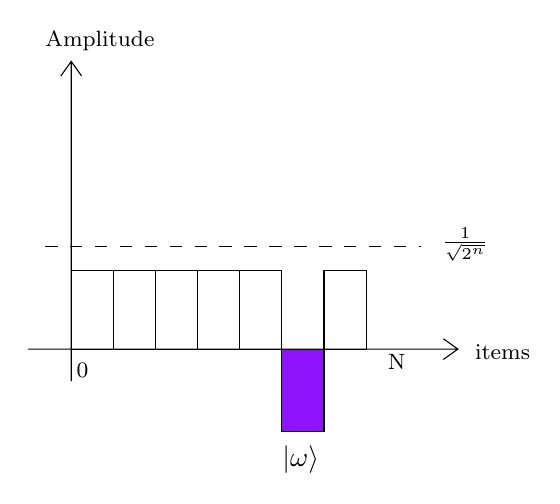
\begin{tikzpicture}[x=0.75pt,y=0.75pt,yscale=-1,xscale=1]
        %uncomment if require: \path (0,421); %set diagram left start at 0, and has height of 421
      
        %Shape: Axis 2D [id:dp13230548671390374] 
      \draw  (388,254.6) -- (595,254.6)(408.7,116) -- (408.7,270) (588,249.6) -- (595,254.6) -- (588,259.6) (403.7,123) -- (408.7,116) -- (413.7,123)  ;
%Shape: Rectangle [id:dp05277599517068765] 
\draw   (408.7,216.67) -- (429,216.67) -- (429,254.6) -- (408.7,254.6) -- cycle ;
%Shape: Rectangle [id:dp9567149694615606] 
\draw   (429,216.67) -- (449.3,216.67) -- (449.3,254.6) -- (429,254.6) -- cycle ;
%Shape: Rectangle [id:dp33156724904270707] 
\draw   (449.3,216.67) -- (469.6,216.67) -- (469.6,254.6) -- (449.3,254.6) -- cycle ;
%Shape: Rectangle [id:dp7921289702689205] 
\draw   (469.6,216.67) -- (489.9,216.67) -- (489.9,254.6) -- (469.6,254.6) -- cycle ;
%Shape: Rectangle [id:dp7099186384950043] 
\draw   (489.9,216.67) -- (510.2,216.67) -- (510.2,254.6) -- (489.9,254.6) -- cycle ;
%Shape: Rectangle [id:dp6243887993660082] 
\draw  [fill={rgb, 255:red, 144; green, 19; blue, 254 }  ,fill opacity=1 ] (510.2,254.6) -- (530.5,254.6) -- (530.5,294.33) -- (510.2,294.33) -- cycle ;
%Shape: Rectangle [id:dp9966482917344106] 
\draw   (530.5,216.67) -- (550.8,216.67) -- (550.8,254.6) -- (530.5,254.6) -- cycle ;
%Shape: Rectangle [id:dp29247452792340645] 
\draw  [dash pattern={on 4.5pt off 4.5pt}]  (396.13,205) -- (577.13,205) ;
        
        % Text Node
        \draw (395,100) node [anchor=north west][inner sep=0.75pt]   [align=left] {{\footnotesize Amplitude}};
        % Text Node
        \draw (410,260) node [anchor=north west][inner sep=0.75pt]   [align=left] {{\footnotesize 0}};
        % Text Node
        \draw (586,195) node [anchor=north west][inner sep=0.75pt]  [font=\footnotesize]  {$\frac{1}{\sqrt{2^{n}}}$};
        % Text Node
        \draw (560,256) node [anchor=north west][inner sep=0.75pt]   [align=left] {{\footnotesize N}};
        % Text Node
        \draw (602,251) node [anchor=north west][inner sep=0.75pt]   [align=left] {{\footnotesize items}};
        % Text Node
        \draw (509.2,300) node [anchor=north west][inner sep=0.75pt]    {$\ket{\omega }$};
    
      \end{tikzpicture}
      
      \caption{\label{fig:grover_step_2b} Grover's Algorithm Step 2b}
  \end{subfigure}
  \caption{\label{fig:grover_step_2} Grover's Algorithm Step 2}
\end{figure}
\vspace{5mm}

The reflection oracle $U_\omega$ can be expressed as:
\vspace{5mm}

\begin{equation}
U_\omega = 1 - 2\ket{\omega}\bra{\omega}    
\end{equation}

\vspace{5mm}

\begin{equation}
U_\omega \ket{s} = -\sin\theta\ket{\omega} +  \cos\theta\ket{\omega}    
\end{equation} 
\vspace{5mm}

\noindent
$U_{{\omega }}$ is a reflection at the hyperplane orthogonal to $\ket{\omega}$  for vectors in the plane spanned by $\ket{s'}$  and $\ket{\omega}$\cite{noauthor_grovers_2022}.
\vspace{5mm}

\noindent
Referring to Figure \ref{fig:grover_step_2a}, $\ket{s}$ is reflected about $\ket{s'}$. The reflection operation on $\ket{s}$ in the negative amplitude causes the overall positive average amplitude to decrease slightly as indicated by Figure \ref{fig:grover_step_2b}. 
\pagebreak

\textbf{Step 3:}
\vspace{5mm}

\begin{figure}[h]
  \begin{subfigure}{.5\textwidth}
    \centering
    \tikzset{every picture/.style={line width=0.75pt}} %set default line width to 0.75pt        

    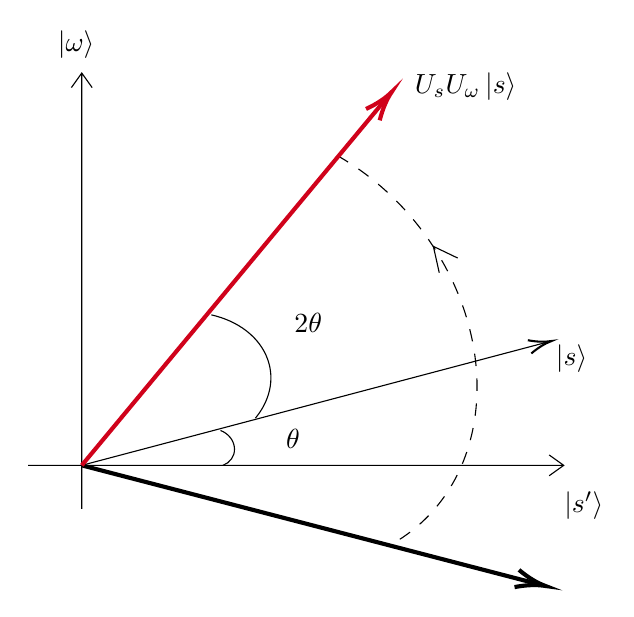
\begin{tikzpicture}[x=0.75pt,y=0.75pt,yscale=-1,xscale=1]
      %uncomment if require: \path (0,421); %set diagram left start at 0, and has height of 421

      %Shape: Axis 2D [id:dp1077584187321754] 
      \draw  (50,245) -- (308,245)(75.8,56) -- (75.8,266) (301,240) -- (308,245) -- (301,250) (70.8,63) -- (75.8,56) -- (80.8,63)  ;
      %Shape: Boxed Line [id:dp16066044861623174] 
      \draw    (75.8,245) -- (300.2,185.61) ;
      \draw [shift={(302.13,185.1)}, rotate = 165.18] [color={rgb, 255:red, 0; green, 0; blue, 0 }  ][line width=0.75]    (10.93,-3.29) .. controls (6.95,-1.4) and (3.31,-0.3) .. (0,0) .. controls (3.31,0.3) and (6.95,1.4) .. (10.93,3.29)   ;
      %Shape: Boxed Line [id:dp9706672155769875] 
      \draw [draw opacity=1 ][fill opacity=1 ][line width=1.5]    (75.8,245) -- (296.23,302.34) ;
      \draw [shift={(299.13,303.1)}, rotate = 194.58] [draw opacity=1 ][line width=1.5]    (14.21,-4.28) .. controls (9.04,-1.82) and (4.3,-0.39) .. (0,0) .. controls (4.3,0.39) and (9.04,1.82) .. (14.21,4.28)   ;
      %Shape: Arc [id:dp872952775851549] 
      \draw  [draw opacity=0][dash pattern={on 4.5pt off 4.5pt}] (198.95,95.79) .. controls (242.68,120.59) and (271.35,171.76) .. (265.48,219.88) .. controls (261.92,249.01) and (246.41,271.27) .. (224.47,283.34) -- (164.47,187.12) -- cycle ; \draw  [dash pattern={on 4.5pt off 4.5pt}] (198.95,95.79) .. controls (242.68,120.59) and (271.35,171.76) .. (265.48,219.88) .. controls (261.92,249.01) and (246.41,271.27) .. (224.47,283.34) ;  
      \draw   (248.03,152.19) -- (245.19,139.5) -- (256.91,145.12) ;
      %Shape: Arc [id:dp6976856692056519] 
      \draw  [draw opacity=0] (142.64,228.2) .. controls (146.47,229.64) and (149.27,233.11) .. (149.38,237.04) .. controls (149.48,240.72) and (147.19,243.77) .. (143.81,245.01) -- (139.59,236.56) -- cycle ; \draw   (142.64,228.2) .. controls (146.47,229.64) and (149.27,233.11) .. (149.38,237.04) .. controls (149.48,240.72) and (147.19,243.77) .. (143.81,245.01) ;  
      %Shape: Boxed Line [id:dp005988885245785669] 
      \draw [color={rgb, 255:red, 208; green, 2; blue, 27 }  ,draw opacity=1 ][fill={rgb, 255:red, 74; green, 144; blue, 226 }  ,fill opacity=1 ][line width=1.5]    (75.8,245) -- (223.22,67.41) ;
      \draw [shift={(225.13,65.1)}, rotate = 129.7] [color={rgb, 255:red, 208; green, 2; blue, 27 }  ,draw opacity=1 ][line width=1.5]    (14.21,-4.28) .. controls (9.04,-1.82) and (4.3,-0.39) .. (0,0) .. controls (4.3,0.39) and (9.04,1.82) .. (14.21,4.28)   ;
      %Shape: Arc [id:dp47337907989211914] 
      \draw  [draw opacity=0] (138.23,172.51) .. controls (151.09,175.41) and (161.57,183.15) .. (165.41,194.07) .. controls (168.83,203.79) and (166.27,214) .. (159.46,222.26) -- (123.73,205.22) -- cycle ; \draw   (138.23,172.51) .. controls (151.09,175.41) and (161.57,183.15) .. (165.41,194.07) .. controls (168.83,203.79) and (166.27,214) .. (159.46,222.26) ;  

      % Text Node
      \draw (63,34.4) node [anchor=north west][inner sep=0.75pt]    {$\ket{\omega }$};
      % Text Node
      \draw (303,185.4) node [anchor=north west][inner sep=0.75pt]    {$\ket{s}$};
      % Text Node
      \draw (307,256.4) node [anchor=north west][inner sep=0.75pt]    {$\ket{s'}$};
      % Text Node
      \draw (173,226.4) node [anchor=north west][inner sep=0.75pt]    {$\theta $};
      % Text Node
      \draw (235,54.4) node [anchor=north west][inner sep=0.75pt]    {$U_{s} U_{\omega }\ket{s}$};
      % Text Node
      \draw (177,170.4) node [anchor=north west][inner sep=0.75pt]    {$2\theta $};

    \end{tikzpicture}
    \caption{\label{fig:grover_step_3a} Grover's Algorithm Step 3a}
  \end{subfigure}%
  \begin{subfigure}{.5\textwidth}
    \centering
    \tikzset{every picture/.style={line width=0.75pt}} %set default line width to 0.75pt        

    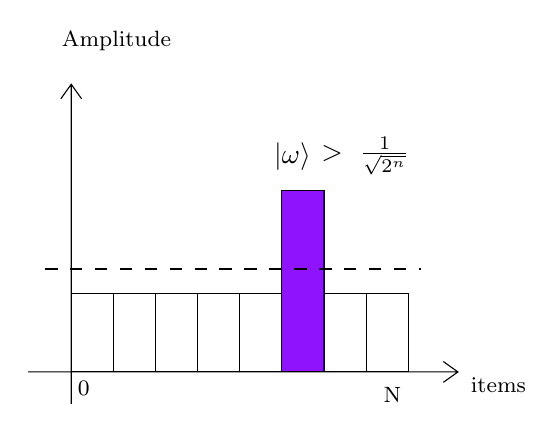
\begin{tikzpicture}[x=0.75pt,y=0.75pt,yscale=-1,xscale=1]
      %uncomment if require: \path (0,421); %set diagram left start at 0, and has height of 421

      %Shape: Axis 2D [id:dp9734077209252769] 
      \draw  (390,249.6) -- (597,249.6)(410.7,111) -- (410.7,265) (590,244.6) -- (597,249.6) -- (590,254.6) (405.7,118) -- (410.7,111) -- (415.7,118)  ;
      %Shape: Rectangle [id:dp3704883525061837] 
      \draw   (410.7,211.67) -- (431,211.67) -- (431,249.6) -- (410.7,249.6) -- cycle ;
      %Shape: Rectangle [id:dp044532975443389855] 
      \draw   (431,211.67) -- (451.3,211.67) -- (451.3,249.6) -- (431,249.6) -- cycle ;
      %Shape: Rectangle [id:dp7877425682227512] 
      \draw   (451.3,211.67) -- (471.6,211.67) -- (471.6,249.6) -- (451.3,249.6) -- cycle ;
      %Shape: Rectangle [id:dp9424861909526165] 
      \draw   (471.6,211.67) -- (491.9,211.67) -- (491.9,249.6) -- (471.6,249.6) -- cycle ;
      %Shape: Rectangle [id:dp22778928407890264] 
      \draw   (491.9,211.67) -- (512.2,211.67) -- (512.2,249.6) -- (491.9,249.6) -- cycle ;
      %Shape: Rectangle [id:dp5422997780895953] 
      \draw  [fill={rgb, 255:red, 144; green, 19; blue, 254 }  ,fill opacity=1 ] (512.2,249.6) -- (532.5,249.6) -- (532.5,162) -- (512.2,162) -- cycle ;
      %Shape: Rectangle [id:dp7263987108332439] 
      \draw   (532.5,211.67) -- (552.8,211.67) -- (552.8,249.6) -- (532.5,249.6) -- cycle ;
      %Shape: Rectangle [id:dp5179786757543001] 
      \draw   (552.8,211.67) -- (573.1,211.67) -- (573.1,249.6) -- (552.8,249.6) -- cycle ;
      %Straight Lines [id:da21954100641972407] 
      \draw  [dash pattern={on 4.5pt off 4.5pt}]  (398.13,200) -- (579.13,200) ;

      % Text Node
      \draw (405,84) node [anchor=north west][inner sep=0.75pt]   [align=left] {{\footnotesize Amplitude}};
      % Text Node
      \draw (412.7,252.6) node [anchor=north west][inner sep=0.75pt]   [align=left] {{\footnotesize 0}};
      % Text Node
      \draw (560,256) node [anchor=north west][inner sep=0.75pt]   [align=left] {{\footnotesize N}};
      % Text Node
      \draw (602,251) node [anchor=north west][inner sep=0.75pt]   [align=left] {{\footnotesize items}};
      % Text Node
      \draw (507.2,138.07) node [anchor=north west][inner sep=0.75pt]    {$\ket{\omega }$};
      % Text Node
      \draw (530,135) node [anchor=north west][inner sep=0.75pt]    {$ >\ \frac{1}{\sqrt{2^{n}}}$};

    \end{tikzpicture}
    \caption{\label{fig:grover_step_3b} Grover's Algorithm Step 3b}
  \end{subfigure}
  \caption{\label{fig:grover_step_3} Grover's Algorithm Step 3}
\end{figure}
\vspace{10mm}

\noindent
As indicated in Figure \ref{fig:grover_step_3a}, a diffusion operator $U_s$ is applied which results in a rotation of $\ket{s}$ by $2\theta$. 
\pagebreak


\begin{figure}
  \begin{center}
      
    \tikzset{every picture/.style={line width=0.75pt}} %set default line width to 0.75pt        

    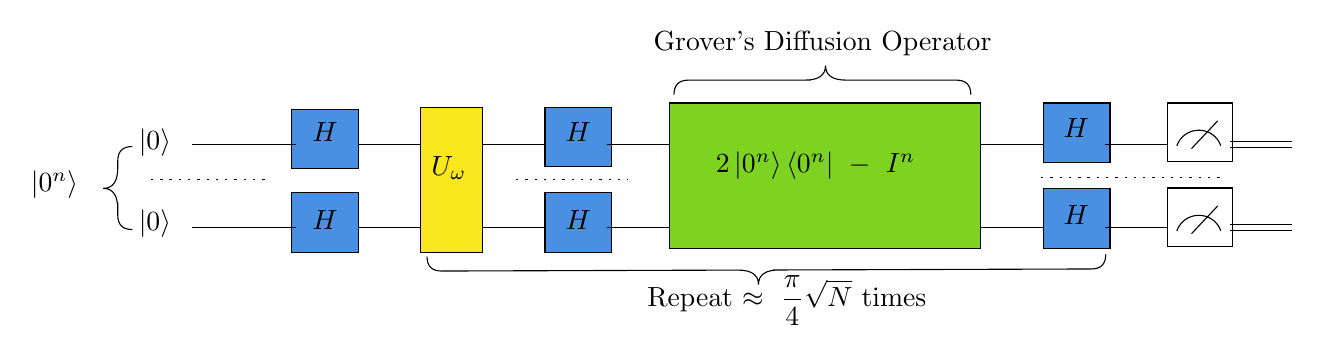
\begin{tikzpicture}[x=0.75pt,y=0.75pt,yscale=-1,xscale=1]
    %uncomment if require: \path (0,392); %set diagram left start at 0, and has height of 392

    %Shape: Rectangle [id:dp8937257723636158] 
    \draw  [fill={rgb, 255:red, 74; green, 144; blue, 226 }  ,fill opacity=1 ] (143,134) -- (175.19,134) -- (175.19,162.7) -- (143,162.7) -- cycle ;
    %Shape: Rectangle [id:dp007021083049765675] 
    \draw  [fill={rgb, 255:red, 74; green, 144; blue, 226 }  ,fill opacity=1 ] (143,174.3) -- (175.19,174.3) -- (175.19,203) -- (143,203) -- cycle ;
    %Shape: Rectangle [id:dp8911339020880464] 
    \draw  [fill={rgb, 255:red, 248; green, 231; blue, 28 }  ,fill opacity=1 ] (205,133) -- (235,133) -- (235,203) -- (205,203) -- cycle ;
    %Shape: Rectangle [id:dp25845825302570513] 
    \draw  [fill={rgb, 255:red, 74; green, 144; blue, 226 }  ,fill opacity=1 ] (265,133) -- (297.19,133) -- (297.19,161.7) -- (265,161.7) -- cycle ;
    %Shape: Rectangle [id:dp47274224679471666] 
    \draw  [fill={rgb, 255:red, 74; green, 144; blue, 226 }  ,fill opacity=1 ] (265,174.3) -- (297.19,174.3) -- (297.19,203) -- (265,203) -- cycle ;
    %Shape: Rectangle [id:dp5929473120919728] 
    \draw  [fill={rgb, 255:red, 126; green, 211; blue, 33 }  ,fill opacity=1 ] (325,131) -- (475,131) -- (475,201) -- (325,201) -- cycle ;
    %Shape: Rectangle [id:dp561230971836093] 
    \draw  [fill={rgb, 255:red, 74; green, 144; blue, 226 }  ,fill opacity=1 ] (505,131) -- (537.19,131) -- (537.19,159.7) -- (505,159.7) -- cycle ;
    %Shape: Rectangle [id:dp551714500077588] 
    \draw  [fill={rgb, 255:red, 74; green, 144; blue, 226 }  ,fill opacity=1 ] (505,172.3) -- (537.19,172.3) -- (537.19,201) -- (505,201) -- cycle ;
    %Shape: Rectangle [id:dp014371224119280157] 
    \draw   (565,131) -- (596.33,131) -- (596.33,159.22) -- (565,159.22) -- cycle ;
    %Shape: Arc [id:dp45728741367881365] 
    \draw  [draw opacity=0] (569.39,151.72) .. controls (570.82,147.31) and (575.03,144.13) .. (579.99,144.13) .. controls (584.9,144.13) and (589.07,147.24) .. (590.55,151.57) -- (579.99,155.06) -- cycle ; \draw   (569.39,151.72) .. controls (570.82,147.31) and (575.03,144.13) .. (579.99,144.13) .. controls (584.9,144.13) and (589.07,147.24) .. (590.55,151.57) ;  
    %Straight Lines [id:da3994764524189143] 
    \draw    (576.46,153) -- (589.1,139.61) ;
    %Shape: Rectangle [id:dp7321580418061253] 
    \draw   (565,172) -- (596.33,172) -- (596.33,200.22) -- (565,200.22) -- cycle ;
    %Shape: Arc [id:dp575518695312089] 
    \draw  [draw opacity=0] (569.39,192.72) .. controls (570.82,188.31) and (575.03,185.13) .. (579.99,185.13) .. controls (584.9,185.13) and (589.07,188.24) .. (590.55,192.57) -- (579.99,196.06) -- cycle ; \draw   (569.39,192.72) .. controls (570.82,188.31) and (575.03,185.13) .. (579.99,185.13) .. controls (584.9,185.13) and (589.07,188.24) .. (590.55,192.57) ;  
    %Straight Lines [id:da9653097238135147] 
    \draw    (576.46,194) -- (589.1,180.61) ;
    %Straight Lines [id:da054926584620969665] 
    \draw    (95,151) -- (145,151) ;
    %Straight Lines [id:da1998461114344101] 
    \draw    (95,191) -- (145,191) ;
    %Straight Lines [id:da13455039306792682] 
    \draw    (175,151) -- (205,151) ;
    %Straight Lines [id:da8941875904744676] 
    \draw    (175,191) -- (205,191) ;
    %Straight Lines [id:da16169269211888615] 
    \draw    (235,151) -- (265,151) ;
    %Straight Lines [id:da6385231938077083] 
    \draw    (235,191) -- (265,191) ;
    %Straight Lines [id:da21590920227006993] 
    \draw    (295,151) -- (325,151) ;
    %Straight Lines [id:da44624469722388915] 
    \draw    (295,191) -- (325,191) ;
    %Straight Lines [id:da9474262709127792] 
    \draw    (475,191) -- (505,191) ;
    %Straight Lines [id:da8304606265085992] 
    \draw    (475,151) -- (505,151) ;
    %Straight Lines [id:da4700710359224989] 
    \draw    (535,151) -- (565,151) ;
    %Straight Lines [id:da09738039485721028] 
    \draw    (535,191) -- (565,191) ;
    %Straight Lines [id:da7131108234298331] 
    \draw    (595,149.5) -- (625,149.5)(595,152.5) -- (625,152.5) ;
    %Straight Lines [id:da9226246067589841] 
    \draw    (595,189.5) -- (625,189.5)(595,192.5) -- (625,192.5) ;
    %Shape: Brace [id:dp5786954336630095] 
    \draw   (208.13,205) .. controls (208.15,209.67) and (210.49,211.99) .. (215.16,211.98) -- (357.81,211.53) .. controls (364.48,211.51) and (367.82,213.83) .. (367.83,218.5) .. controls (367.82,213.83) and (371.14,211.49) .. (377.81,211.47)(374.81,211.48) -- (528.16,210.99) .. controls (532.83,210.98) and (535.15,208.64) .. (535.13,203.97) ;
    %Shape: Brace [id:dp3814057437492582] 
    \draw   (470.13,127) .. controls (470.13,122.33) and (467.8,120) .. (463.13,120) -- (410.13,120) .. controls (403.46,120) and (400.13,117.67) .. (400.13,113) .. controls (400.13,117.67) and (396.8,120) .. (390.13,120)(393.13,120) -- (334.13,120) .. controls (329.46,120) and (327.13,122.33) .. (327.13,127) ;
    %Shape: Brace [id:dp5248227356988384] 
    \draw   (66.13,152) .. controls (61.46,152) and (59.13,154.33) .. (59.13,159) -- (59.13,162.16) .. controls (59.13,168.83) and (56.8,172.16) .. (52.13,172.16) .. controls (56.8,172.16) and (59.13,175.49) .. (59.13,182.16)(59.13,179.16) -- (59.13,185) .. controls (59.13,189.67) and (61.46,192) .. (66.13,192) ;
    %Straight Lines [id:da6246903517915476] 
    \draw  [dash pattern={on 0.84pt off 2.51pt}]  (75.13,168) -- (133.13,168) ;
    %Straight Lines [id:da7651260164716407] 
    \draw  [dash pattern={on 0.84pt off 2.51pt}]  (251,168) -- (305.13,168) ;
    %Straight Lines [id:da5357419850229155] 
    \draw  [dash pattern={on 0.84pt off 2.51pt}]  (504,167) -- (592.13,167) ;

    % Text Node
    \draw (151.6,139.4) node [anchor=north west][inner sep=0.75pt]    {$H$};
    % Text Node
    \draw (151.6,181.4) node [anchor=north west][inner sep=0.75pt]    {$H$};
    % Text Node
    \draw (209,155.4) node [anchor=north west][inner sep=0.75pt]    {$U_{\omega }$};
    % Text Node
    \draw (273.6,139.4) node [anchor=north west][inner sep=0.75pt]    {$H$};
    % Text Node
    \draw (273.6,181.4) node [anchor=north west][inner sep=0.75pt]    {$H$};
    % Text Node
    \draw (513.6,137.4) node [anchor=north west][inner sep=0.75pt]    {$H$};
    % Text Node
    \draw (513.6,179.4) node [anchor=north west][inner sep=0.75pt]    {$H$};
    % Text Node
    \draw (346,153.4) node [anchor=north west][inner sep=0.75pt]    {$2\ket{0^{n}}\bra{0^{n}} \ -\ I^{n}$};
    % Text Node
    \draw (68,142.4) node [anchor=north west][inner sep=0.75pt]    {$\ket{0}$};
    % Text Node
    \draw (68,181.4) node [anchor=north west][inner sep=0.75pt]    {$\ket{0}$};
    % Text Node
    \draw (16,162.4) node [anchor=north west][inner sep=0.75pt]    {$\ket{0^{n}}$};
    % Text Node
    \draw (316,95) node [anchor=north west][inner sep=0.75pt]   [align=left] {Grover's Diffusion Operator};
    % Text Node
    \draw (313,213) node [anchor=north west][inner sep=0.75pt]   [align=left] {Repeat $\displaystyle \approx \ \frac{\pi }{4}\sqrt{N}$ times};

    \end{tikzpicture}
  \end{center}

  \caption{\label{fig:grover_circuit} Quantum circuit representation of Grover's Algorithm.}
\end{figure}

\vspace{5mm}


\noindent
The diffusion operator is expressed as:
\vspace{5mm}

\begin{equation}
U_s  = 2 \ket{s}\bra{s} - 1    
\end{equation}
\vspace{5mm}

\noindent
$U_s$ is a reflection at the hyperplane orthogonal to $\ket{\perp s}$  for vectors in the plane spanned by $\ket{s}$  and $\ket{\perp s}$, in other words a reflection about $\ket{s}$. 
\vspace{5mm}

\noindent
The product of two reflection operators $U_\omega$ and $U_s$ is a rotation in the plane spanned by $\ket{\omega}$ and $\ket{s'}$ through twice the angle $\theta$.
\vspace{5mm}

\noindent
By applying $U_s$ and $U_\omega$ the initial state $\ket{s}$ is rotated close to the state $\ket{\omega}$.
\vspace{5mm}

\noindent
After repeated Grover iterations, $\ket{s}$ approaches $\ket{\omega}$, at which point an observation in the computational basis
outputs a solution to the search problem with high probability.
\vspace{5mm}

\noindent
By looking at Figure \ref{fig:grover_step_3b}, the amplitude of $\ket{\omega}$ is reflected about the average amplitude. Referring to Figure \ref{fig:grover_step_2b}, the average amplitude is lowered below the dashed line and the reflection boosts the amplitude by about three times its original value, as depicted in Figure \ref{fig:grover_step_3b}.
\vspace{5mm}

\noindent
Step 2 and Step 3 will be repeated where necessary for $T$ times until the average amplitude approaches zero so that the amplitude for $\ket{\omega} \sim 1$\cite{de_wolf_main_nodate}.
\vspace{5mm}

\noindent
By observation, the number of times $T$ is required to apply the Grover's Algorithm according to Figure \ref{fig:grover_step_3a} can be written as:
\vspace{5mm}

\noindent
\begin{equation}
\theta_T = (2T + 1)\theta
\end{equation}

Where $\theta_T \approx \frac{\pi}{2}$ and $T$ is chosen to the nearest integer. 
\pagebreak

\noindent
For an unstructured search through a sufficiently large list, $\theta$ will be small. Using the small angle approximation, $\sin\theta \approx \theta$. 
\vspace{5mm}

\noindent
Recall that $\sin\theta = \frac{1}{\sqrt{2^n}}$
\vspace{5mm}

\noindent
Hence:
\vspace{5mm}

\noindent
\begin{equation}
T \approx \frac{\pi}{4\theta} \approx \frac{\pi}{4}\sqrt{2^n}    
\end{equation}

Note that $N = 2^n$ has been used interchangeably in this literature.
\vspace{5mm}

\noindent
Consequently, it is shown that $T$ is directly proportional to the order $O(\sqrt{N})$.
\vspace{5mm}

\noindent
In terms of the amplitude of the state $\ket{s}$, it is observed to grow linearly with the number of application of $\sim T\sqrt{N}$. Therefore the amplitude and the probability are both amplified in Grover's Algorithm.
\vspace{5mm}

\noindent
For multiple search entries $M$, the number of Grover's iteration would be roughly $\sqrt{\frac{N}{M}}$.
\vspace{10mm}

\subsection{Advantages and Disadvantages}
\vspace{5mm}

\noindent
The obvious advantage of the Grover's Algorithm is the quadratic speed up over classical search algorithms. 
\vspace{5mm}

\noindent
In the previous chapter, Grover's Algorithm shows amplitude amplification on the target state $\ket{\omega}$ and this can be used to speed up a wide variety of other algorithms\cite{noauthor_grovers_nodate}. 
\vspace{5mm}

\noindent
One of the few drawbacks of the Grover's Algorithm is that it is probabilistic. However the probability error can be significantly reduced by repeating the algorithm.
\vspace{5mm}

\noindent
Due to the constraints of currently available quantum computers, Grover's Algorithm is yet to yield any  meaningful quadratic speed up compared to classical algorithms\cite{noauthor_grovers_2022}.   
\pagebreak

\section{Phase Estimation}
\subsection{Introduction}
Suppose you have a unitary operator $U$ and its eigenvector $\ket{u}$ with eigenvalue $e^{2\pi i \phi}$, with $\phi$ unknown. By performing phase estimation, we can estimate $\phi$ (exact if the decimal expansion of $\phi$ is finite), up to required precision $n$. Phase estimation is needed for the algorithm of order-finding and it's extension, Shor's factoring algorithm. The figure below illustrate this process.

\vspace{5mm}

\tikzset{every picture/.style={line width=0.75pt}} %set default line width to 0.75pt        

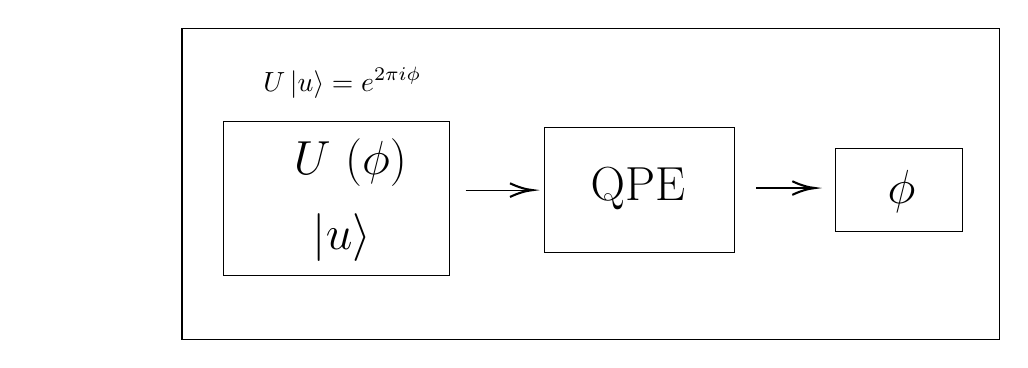
\begin{tikzpicture}[x=0.75pt,y=0.75pt,yscale=-1,xscale=1]
\path (0,195); %set diagram left start at 0, and has height of 300

%Shape: Rectangle [id:dp5239908419271088] 
\draw   (249,94) -- (340.33,94) -- (340.33,154) -- (249,154) -- cycle ;
%Shape: Rectangle [id:dp798673162776731] 
\draw   (94.33,91) -- (203.33,91) -- (203.33,165) -- (94.33,165) -- cycle ;
%Straight Lines [id:da0439097804330606] 
\draw    (211,124) -- (241.33,124) ;
\draw [shift={(243.33,124)}, rotate = 180] [color={rgb, 255:red, 0; green, 0; blue, 0 }  ][line width=0.75]    (10.93,-3.29) .. controls (6.95,-1.4) and (3.31,-0.3) .. (0,0) .. controls (3.31,0.3) and (6.95,1.4) .. (10.93,3.29)   ;
%Straight Lines [id:da053999006588390186] 
\draw    (351,123) -- (377.33,123) ;
\draw [shift={(379.33,123)}, rotate = 180] [color={rgb, 255:red, 0; green, 0; blue, 0 }  ][line width=0.75]    (10.93,-3.29) .. controls (6.95,-1.4) and (3.31,-0.3) .. (0,0) .. controls (3.31,0.3) and (6.95,1.4) .. (10.93,3.29)   ;
%Shape: Rectangle [id:dp5103744878863842] 
\draw   (389,104) -- (450.33,104) -- (450.33,144) -- (389,144) -- cycle ;
%Shape: Rectangle [id:dp6849328641759378] 
\draw   (74.33,46) -- (468.33,46) -- (468.33,196) -- (74.33,196) -- cycle ;

% Text Node
\draw (270,112) node [anchor=north west][inner sep=0.75pt]  [font=\LARGE] [align=left] {QPE};
% Text Node
\draw (127,98) node [anchor=north west][inner sep=0.75pt]   [align=left][font=\LARGE] {$\displaystyle U\ ( \phi )$};
% Text Node
\draw (112,63) node [anchor=north west][inner sep=1pt]   [align=left]{$\displaystyle U\ket{u} =e^{2\pi i\phi }$};
% Text Node
\draw (136,134) node [anchor=north west][inner sep=0.75pt] [font=\LARGE]  [align=left] {$\displaystyle \ket{u}$};
% Text Node
\draw (413,113) node [anchor=north west][inner sep=0.75pt][font=\LARGE]   [align=left] {$\displaystyle \phi $};


\end{tikzpicture}
\begin{center}
    Phase Estimation (abbreviated as QPE).
\end{center}  

\subsection{Quantum Fourier Transform}
To implement the phase estimation algorithm, the key ingredient is the quantum Fourier transform. Quantum Fourier transform is analogous to the classical discrete Fourier transform, where the basis of a vector is changed into another basis that is useful for computation or analysis. The effect of quantum Fourier transform on an arbitrary state vector can be summarised as below \cite{nielsen_quantum_2010}:
\begin{equation}
    \ket{v} = \frac{1}{\sqrt{N}} \sum_{i=0}^{N-1}{x_i \ket{i}} \xRightarrow{QFT} \ket{\Tilde{v}} = \frac{1}{\sqrt{N}}\sum_{j=0}^{N-1} y_j \ket{j}
\end{equation} 

\noindent
Note that only the amplitudes of the eigenstates are affected by this transformation. Similar to Fourier transform which decomposes functions depending on space or time into functions depending on spatial frequency or temporal frequency, QFT maps the computational basis states between the $\hat{\textbf{z}}$-basis states to the $\hat{\textbf{x}}$-basis states.
\vspace{5mm}

\noindent
The $\hat{\textbf{x}}$-basis states are defined as:
\vspace{5mm}
\begin{equation}
\ket{+} = \frac{1}{\sqrt{2}}(\ket{0} + \ket{1}) \ \text{and} \ \ket{-} = \frac{1}{\sqrt{2}}(\ket{0} - \ket{1})   
\end{equation}

\vspace{5mm}

\noindent
For multi-qubit states in the computational basis have corresponding states in the Fourier basis. The QFT is the function that transforms between these bases\cite{noauthor_quantum_nodate-1}:
\vspace{5mm}

\begin{equation}
\ket{\text{State in computational basis}} \rightarrow{\text{QFT}} \ket{\text{State in Fourier basis}}  
\end{equation}
\vspace{5mm}

\qquad $\text{QFT}\ket{x} = \ket{\tilde{x}}$
\vspace{5mm}

For a $n$ qubit states, the QFT has the effect of \cite{nielsen_quantum_2010}:
\vspace{5mm}
\begin{equation}
\text{QFT}_N\ket{x} = \frac{1}{\sqrt{N}} \sum\limits_{y=0}^{N-1}e^{2i\pi\frac{xy}{2^n}}\ket{y} \ , \ \text{for} \ N = 2^n    
\end{equation}

\vspace{5mm}

\begin{equation}
=  \frac{1}{\sqrt{N}} \sum\limits_{y=0}^{N-1}e^{2i\pi x(\sum_{k=1}^{n}\frac{y_k}{2^k})}\ket{y...y_n} 
\end{equation}
\vspace{5mm}

Rewriting $y$ in binary fraction $y= y_1 ... y_n, \frac{y}{2^n} = \sum\limits_{k=1}^{n}\frac{y_k}{2^k}$   
\vspace{5mm}

\begin{equation}
= \frac{1}{\sqrt{N}} \sum\limits_{y=0}^{N-1}\prod\limits_{k=1}^{n}e^{2i\pi x\frac{y_k}{2^k}}\ket{y...y_n}    
\end{equation}
\vspace{5mm}

\noindent
After expanding the exponential of a sum to a product of exponentials.
\vspace{5mm}

\begin{equation}
= \frac{1}{\sqrt{N}}\bigotimes\limits_{k=1}^{n}(\ket{0} + e^{\frac{2i\pi x}{2^k}}\ket{1})  
\end{equation}
\vspace{5mm}

\noindent
After rearranging the sum and products, and expanding $\sum\limits_{y=0}^{N-1} = \sum\limits_{y_1=0}^{1}\sum\limits_{y_2=0}^{1}...\sum\limits_{y_0=0}^{1} $
\vspace{5mm}

\begin{equation}
= \frac{1}{\sqrt{N}}(\ket{0} + e^{\frac{2i\pi x}{2}}\ket{1}) \bigotimes (\ket{0} + e^{\frac{2i\pi x}{2^2}}\ket{1}) \bigotimes ... \bigotimes(\ket{0} + e^{\frac{2i\pi x}{2^{n-1}}}\ket{1}) \bigotimes (\ket{0} + e^{\frac{2i\pi x}{2^n}}\ket{1})    
\end{equation}
\pagebreak

The circuit to implement QFT for a n-qubit state is shown below
\vspace{5mm}

\noindent


\begin{figure}[h]
    \centering
\tikzset{every picture/.style={line width=0.75pt}} %set default line width to 0.75pt        


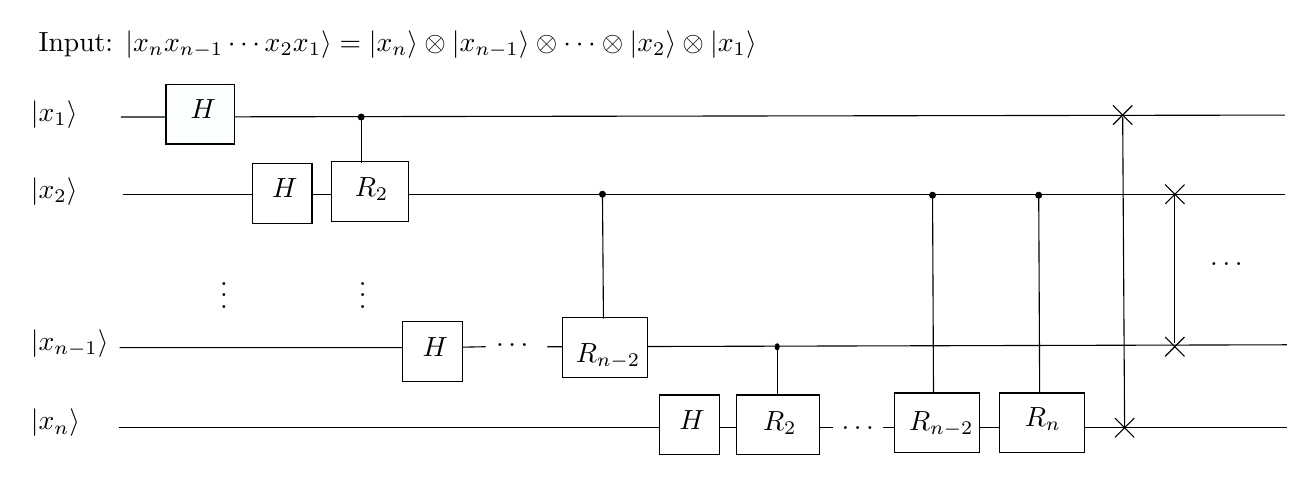
\begin{tikzpicture}[x=0.75pt,y=0.75pt,yscale=-0.93,xscale=0.93]
\path (0,205); %set diagram left start at 0, and has height of 300

%Straight Lines [id:da7550574313481198] 
\draw    (442,212) -- (651,212) ;
%Straight Lines [id:da6398571931609234] 
\draw    (46,212) -- (210.17,212) -- (416,212) ;
%Straight Lines [id:da8727674531656819] 
\draw    (46.35,170.5) -- (210.51,170.5) -- (236,170) ;
%Straight Lines [id:da8871926231699048] 
\draw    (48,91) -- (650,91) ;
%Straight Lines [id:da28106686876999853] 
\draw    (47,51) -- (650,50) ;
%Shape: Rectangle [id:dp9740729644202252] 
\draw  [fill={rgb, 255:red, 255; green, 255; blue, 255 }  ,fill opacity=1 ] (114.97,75) -- (146,75) -- (146,106) -- (114.97,106) -- cycle ;

%Shape: Rectangle [id:dp426089737124529] 
\draw  [fill={rgb, 255:red, 255; green, 255; blue, 255 }  ,fill opacity=1 ] (193,157) -- (224.03,157) -- (224.03,188) -- (193,188) -- cycle ;

%Shape: Rectangle [id:dp8514934588123941] 
\draw  [fill={rgb, 255:red, 255; green, 255; blue, 255 }  ,fill opacity=1 ] (326,195) -- (357.03,195) -- (357.03,226) -- (326,226) -- cycle ;

%Shape: Rectangle [id:dp314360945613794] 
\draw  [fill={rgb, 255:red, 255; green, 255; blue, 255 }  ,fill opacity=1 ] (156,74) -- (196,74) -- (196,105) -- (156,105) -- cycle ;

%Straight Lines [id:da39077578043373473] 
\draw    (171.5,75) -- (171.5,51) ;
%Shape: Circle [id:dp441535044324351] 
\draw  [fill={rgb, 255:red, 2; green, 2; blue, 2 }  ,fill opacity=1 ] (170,51) .. controls (170,51.83) and (170.67,52.5) .. (171.5,52.5) .. controls (172.33,52.5) and (173,51.83) .. (173,51) .. controls (173,50.17) and (172.33,49.5) .. (171.5,49.5) .. controls (170.67,49.5) and (170,50.17) .. (170,51) -- cycle ;

%Shape: Rectangle [id:dp5897080780221526] 
\draw  [fill={rgb, 255:red, 252; green, 255; blue, 255 }  ,fill opacity=1 ] (70.37,34) -- (106,34) -- (106,65) -- (70.37,65) -- cycle ;

%Shape: Rectangle [id:dp30473357310759497] 
\draw  [fill={rgb, 255:red, 255; green, 255; blue, 255 }  ,fill opacity=1 ] (366,195) -- (409,195) -- (409,226) -- (366,226) -- cycle ;

%Straight Lines [id:da3855769866550789] 
\draw    (268,170) -- (279.33,170) -- (651,169) ;
%Shape: Rectangle [id:dp9695497040119231] 
\draw  [fill={rgb, 255:red, 255; green, 255; blue, 255 }  ,fill opacity=1 ] (276,155) -- (320,155) -- (320,186) -- (276,186) -- cycle ;
%Straight Lines [id:da42876538848964485] 
\draw    (297,155.5) -- (296.5,91) ;
%Shape: Circle [id:dp5965904538619509] 
\draw  [fill={rgb, 255:red, 2; green, 2; blue, 2 }  ,fill opacity=1 ] (295,91) .. controls (295,91.83) and (295.67,92.5) .. (296.5,92.5) .. controls (297.33,92.5) and (298,91.83) .. (298,91) .. controls (298,90.17) and (297.33,89.5) .. (296.5,89.5) .. controls (295.67,89.5) and (295,90.17) .. (295,91) -- cycle ;

%Straight Lines [id:da8537072100283741] 
\draw    (387,195) -- (387,170.06) ;
%Shape: Ellipse [id:dp044376374855228495] 
\draw  [fill={rgb, 255:red, 2; green, 2; blue, 2 }  ,fill opacity=1 ] (386,170.06) .. controls (386,170.92) and (386.45,171.62) .. (387,171.62) .. controls (387.55,171.62) and (388,170.92) .. (388,170.06) .. controls (388,169.2) and (387.55,168.5) .. (387,168.5) .. controls (386.45,168.5) and (386,169.2) .. (386,170.06) -- cycle ;
%Shape: Rectangle [id:dp1253251355263153] 
\draw  [fill={rgb, 255:red, 255; green, 255; blue, 255 }  ,fill opacity=1 ] (448,194) -- (492,194) -- (492,225) -- (448,225) -- cycle ;
%Shape: Rectangle [id:dp5170244213525657] 
\draw  [fill={rgb, 255:red, 255; green, 255; blue, 255 }  ,fill opacity=1 ] (502,194) -- (546,194) -- (546,225) -- (502,225) -- cycle ;
%Straight Lines [id:da6842415574484656] 
\draw    (468,194) -- (467.5,91.5) ;
%Shape: Circle [id:dp7507766602263973] 
\draw  [fill={rgb, 255:red, 2; green, 2; blue, 2 }  ,fill opacity=1 ] (466,91.5) .. controls (466,92.33) and (466.67,93) .. (467.5,93) .. controls (468.33,93) and (469,92.33) .. (469,91.5) .. controls (469,90.67) and (468.33,90) .. (467.5,90) .. controls (466.67,90) and (466,90.67) .. (466,91.5) -- cycle ;
%Straight Lines [id:da48965934705174585] 
\draw    (523,194) -- (522.5,91.5) ;
%Shape: Circle [id:dp6048474775771464] 
\draw  [fill={rgb, 255:red, 2; green, 2; blue, 2 }  ,fill opacity=1 ] (521,91.5) .. controls (521,92.33) and (521.67,93) .. (522.5,93) .. controls (523.33,93) and (524,92.33) .. (524,91.5) .. controls (524,90.67) and (523.33,90) .. (522.5,90) .. controls (521.67,90) and (521,90.67) .. (521,91.5) -- cycle ;
%Straight Lines [id:da015312271871600447] 
\draw    (566,51) -- (567,212) ;
%Straight Lines [id:da5584559248399006] 
\draw    (593,91) -- (593,168) ;
%Straight Lines [id:da9780974093157568] 
\draw    (561,45) -- (571,55) ;
%Straight Lines [id:da38915226135752146] 
\draw    (571,45) -- (561,55) ;

%Straight Lines [id:da6675236283011767] 
\draw    (562,207) -- (572,217) ;
%Straight Lines [id:da6834744460286415] 
\draw    (572,207) -- (562,217) ;

%Straight Lines [id:da07839335868474284] 
\draw    (588,165) -- (598,175) ;
%Straight Lines [id:da88112867187513] 
\draw    (598,165) -- (588,175) ;

%Straight Lines [id:da04164548314578809] 
\draw    (588,86) -- (598,96) ;
%Straight Lines [id:da5017829132129701] 
\draw    (598,86) -- (588,96) ;


% Text Node
\draw (81.82,40.7) node [anchor=north west][inner sep=0.75pt]   [align=left] {$\displaystyle H$};
% Text Node
\draw (123.97,81.7) node [anchor=north west][inner sep=0.75pt]   [align=left] {$\displaystyle H$};
% Text Node
\draw (202,163.7) node [anchor=north west][inner sep=0.75pt]   [align=left] {$\displaystyle H$};
% Text Node
\draw (335,201.7) node [anchor=north west][inner sep=0.75pt]   [align=left] {$\displaystyle H$};
% Text Node
\draw (166.8,81) node [anchor=north west][inner sep=0.75pt]   [align=left] {$\displaystyle R_{2}$};
% Text Node
\draw (97,127) node [anchor=north west][inner sep=0.75pt]   [align=left] {$\displaystyle \vdots $};
% Text Node
\draw (169,127) node [anchor=north west][inner sep=0.75pt]   [align=left] {$\displaystyle \vdots $};
% Text Node
\draw (378.36,202) node [anchor=north west][inner sep=0.75pt]   [align=left] {$\displaystyle R_{2}$};
% Text Node
\draw (240,167) node [anchor=north west][inner sep=0.75pt]   [align=left] {$\displaystyle \dotsc $};
% Text Node
\draw (281.4,167) node [anchor=north west][inner sep=0.75pt]   [align=left] {$\displaystyle R_{n-2}$};
% Text Node
\draw (419,210) node [anchor=north west][inner sep=0.75pt]   [align=left] {$\displaystyle \dotsc $};
% Text Node
\draw (454,202) node [anchor=north west][inner sep=0.75pt]   [align=left] {$\displaystyle R_{n-2}$};
% Text Node
\draw (514,200) node [anchor=north west][inner sep=0.75pt]   [align=left] {$\displaystyle R_{n}$};
% Text Node
\draw (610,125) node [anchor=north west][inner sep=0.75pt]   [align=left] {$\displaystyle \dotsc $};
% Text Node
\draw (-1,41) node [anchor=north west][inner sep=0.75pt]   [align=left] {$\displaystyle \ket{x_{1}}$};
% Text Node
\draw (-1,81) node [anchor=north west][inner sep=0.75pt]   [align=left] {$\displaystyle \ket{x_{2}}$};
% Text Node
\draw (-1,160) node [anchor=north west][inner sep=0.75pt]   [align=left] {$\displaystyle \ket{x_{n-1}}$};
% Text Node
\draw (-1,201) node [anchor=north west][inner sep=0.75pt]   [align=left] {$\displaystyle \ket{x_{n}}$};
% Text Node
\draw (3,5) node [anchor=north west][inner sep=0.75pt]   [align=left] {Input: $\displaystyle \ket{x_{n} x_{n-1} \cdots x_{2} x_{1}} =\ket{x_{n}} \otimes \ket{x_{n-1}} \otimes \cdots \otimes \ket{x_{2}} \otimes \ket{x_{1}}$};

\end{tikzpicture}
\caption{The QFT Circuit}
\end{figure}
\vspace{5mm}

where $H$ is the Hadamard gate, \(R_n = 
\begin{bmatrix}
    1 & 0 \\
    0 & e^{2\pi i/2^k}
\end{bmatrix} \)
, and the 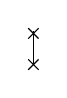
\begin{tikzpicture}[x=0.75pt,y=0.75pt,yscale=0.5,xscale=0.5]
%uncomment if require: \path (0,300); %set diagram left start at 0, and has height of 300

%Straight Lines [id:da5239484844882938] 
\draw    (85,16) -- (85,47) ;
%Straight Lines [id:da8400020556735358] 
\draw    (80,40) -- (90,50) ;
%Straight Lines [id:da24481923694858] 
\draw    (90,40) -- (80,50) ;

%Straight Lines [id:da0676093949143659] 
\draw    (80,10) -- (90,20) ;
%Straight Lines [id:da9539947353268269] 
\draw    (90,10) -- (80,20) ;
\end{tikzpicture} is a swap gate, which swaps the qubit i with the n-i qubit. However, the phase estimation algorithm requires the inverse QFT, which is easy to construct by flipping the circuit horizontally, and conjugate the phases in the $R_k$ gate.
\pagebreak
\subsection{The Algorithm}
The phase estimation procedure uses two registers, with the first register containing $m$ qubits (all in the state $\ket{0}$) and the second register is in the state $\ket{u}$, and contains as many qubits as required for $\ket{u}$. The number of qubits $m$ for first register is dependent on the precision of the phase required, which will be discussed in the next section. The algorithm can be summarized below:\\
i. Hadamard gates are applied to all qubits in first register.\\
ii. Control-U gates raised to successive powers of two is applied consecutively to the second register, with the controls covering the first qubit to the last qubit in the first register.\\
iii. The inverse QFT operation is then applied on the first register to obtain a number, which needs further to be further divided by $2^m$ to recover the estimation of the phase.\\
The circuit below sums up the whole procedure.
\vspace{5mm}


    
\begin{figure}[h]

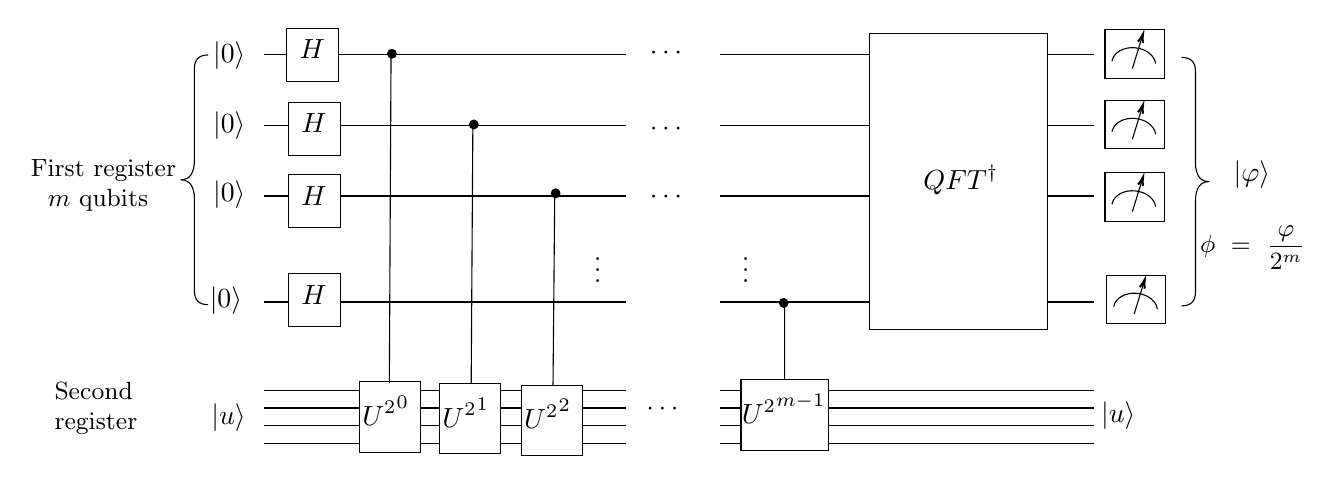
\begin{tikzpicture}[x=0.75pt,y=0.75pt,yscale=-0.95,xscale=0.95]
%uncomment if require: \path (0,255); %set diagram left start at 0, and has height of 255

%Straight Lines [id:da9194835056551176] 
\draw    (120.56,38.44) -- (304.21,38.44) ;
%Straight Lines [id:da6985548639030699] 
\draw    (120.56,74.27) -- (304.21,74.27) ;
%Straight Lines [id:da7116263330867054] 
\draw    (120.56,110.11) -- (304.21,110.11) ;
%Straight Lines [id:da8626589126730531] 
\draw    (120.56,163.86) -- (304.21,163.86) ;
%Straight Lines [id:da19695588367886063] 
\draw    (120.56,208.65) -- (304.21,208.65) ;
%Straight Lines [id:da10938435456147] 
\draw    (120.56,217.61) -- (304.21,217.61) ;
%Straight Lines [id:da4912942246519334] 
\draw    (120.56,226.57) -- (304.21,226.57) ;
%Straight Lines [id:da12940095959327003] 
\draw    (120.56,235.53) -- (304.21,235.53) ;
%Shape: Rectangle [id:dp15884195779468213] 
\draw  [fill={rgb, 255:red, 255; green, 255; blue, 255 }  ,fill opacity=1 ] (132.04,25) -- (158.54,25) -- (158.54,51.88) -- (132.04,51.88) -- cycle ;

%Shape: Rectangle [id:dp23256435967097955] 
\draw  [fill={rgb, 255:red, 255; green, 255; blue, 255 }  ,fill opacity=1 ] (132.93,62.63) -- (159.42,62.63) -- (159.42,89.5) -- (132.93,89.5) -- cycle ;

%Shape: Rectangle [id:dp37562370103024234] 
\draw  [fill={rgb, 255:red, 255; green, 255; blue, 255 }  ,fill opacity=1 ] (132.93,99.36) -- (159.42,99.36) -- (159.42,126.23) -- (132.93,126.23) -- cycle ;

%Shape: Rectangle [id:dp03136015448302287] 
\draw  [fill={rgb, 255:red, 255; green, 255; blue, 255 }  ,fill opacity=1 ] (132.93,149.53) -- (159.42,149.53) -- (159.42,176.4) -- (132.93,176.4) -- cycle ;

%Shape: Rectangle [id:dp03155077547529872] 
\draw  [fill={rgb, 255:red, 255; green, 255; blue, 255 }  ,fill opacity=1 ] (169.1,204.17) -- (200.01,204.17) -- (200.01,240.01) -- (169.1,240.01) -- cycle ;

%Shape: Rectangle [id:dp9729186752169825] 
\draw  [fill={rgb, 255:red, 255; green, 255; blue, 255 }  ,fill opacity=1 ] (209.72,205.07) -- (240.63,205.07) -- (240.63,240.9) -- (209.72,240.9) -- cycle ;
%Shape: Rectangle [id:dp19964985396092239] 
\draw  [fill={rgb, 255:red, 255; green, 255; blue, 255 }  ,fill opacity=1 ] (251.23,205.97) -- (282.14,205.97) -- (282.14,241.8) -- (251.23,241.8) -- cycle ;
%Straight Lines [id:da7109063051521263] 
\draw    (351.93,38.44) -- (541.76,38.44) ;
%Straight Lines [id:da1930170699837772] 
\draw    (351.93,74.27) -- (541.76,74.27) ;
%Straight Lines [id:da7712890300467412] 
\draw    (351.93,110.11) -- (541.76,110.11) ;
%Straight Lines [id:da00469730483476738] 
\draw    (351.93,163.86) -- (541.76,163.86) ;
%Straight Lines [id:da9060427595505647] 
\draw    (351.93,208.65) -- (541.76,208.65) ;
%Straight Lines [id:da24660499214292575] 
\draw    (351.93,217.61) -- (541.76,217.61) ;
%Straight Lines [id:da8073093108188725] 
\draw    (351.93,226.57) -- (541.76,226.57) ;
%Straight Lines [id:da9156311780855882] 
\draw    (351.93,235.53) -- (541.76,235.53) ;
%Shape: Rectangle [id:dp5274524103344703] 
\draw  [fill={rgb, 255:red, 255; green, 255; blue, 255 }  ,fill opacity=1 ] (362.5,203.28) -- (406.65,203.28) -- (406.65,239.11) -- (362.5,239.11) -- cycle ;
%Straight Lines [id:da03444841972411539] 
\draw    (185,39.15) -- (184.14,205.07) ;
%Straight Lines [id:da009404546254211943] 
\draw    (226.5,74.09) -- (225.65,205.07) ;
%Straight Lines [id:da374044199582911] 
\draw    (268.01,110.82) -- (267.15,205.97) ;
%Straight Lines [id:da6555871247561469] 
\draw    (384.57,163.68) -- (384.6,203.28) ;
%Shape: Ellipse [id:dp31242914795993315] 
\draw  [fill={rgb, 255:red, 0; green, 0; blue, 0 }  ,fill opacity=1 ] (183.26,37.98) .. controls (183.26,36.75) and (184.24,35.75) .. (185.45,35.75) .. controls (186.67,35.75) and (187.65,36.75) .. (187.65,37.98) .. controls (187.65,39.2) and (186.67,40.2) .. (185.45,40.2) .. controls (184.24,40.2) and (183.26,39.2) .. (183.26,37.98) -- cycle ;
%Shape: Ellipse [id:dp8473767958403672] 
\draw  [fill={rgb, 255:red, 0; green, 0; blue, 0 }  ,fill opacity=1 ] (224.77,73.81) .. controls (224.77,72.58) and (225.75,71.59) .. (226.96,71.59) .. controls (228.17,71.59) and (229.15,72.58) .. (229.15,73.81) .. controls (229.15,75.04) and (228.17,76.03) .. (226.96,76.03) .. controls (225.75,76.03) and (224.77,75.04) .. (224.77,73.81) -- cycle ;
%Shape: Ellipse [id:dp8148369515275169] 
\draw  [fill={rgb, 255:red, 0; green, 0; blue, 0 }  ,fill opacity=1 ] (266.27,108.75) .. controls (266.27,107.52) and (267.25,106.52) .. (268.46,106.52) .. controls (269.67,106.52) and (270.66,107.52) .. (270.66,108.75) .. controls (270.66,109.98) and (269.67,110.97) .. (268.46,110.97) .. controls (267.25,110.97) and (266.27,109.98) .. (266.27,108.75) -- cycle ;
%Shape: Ellipse [id:dp35408407729589786] 
\draw  [fill={rgb, 255:red, 0; green, 0; blue, 0 }  ,fill opacity=1 ] (381.95,164.29) .. controls (381.95,163.06) and (382.94,162.07) .. (384.15,162.07) .. controls (385.36,162.07) and (386.34,163.06) .. (386.34,164.29) .. controls (386.34,165.52) and (385.36,166.52) .. (384.15,166.52) .. controls (382.94,166.52) and (381.95,165.52) .. (381.95,164.29) -- cycle ;
%Shape: Rectangle [id:dp08709255028482066] 
\draw  [fill={rgb, 255:red, 255; green, 255; blue, 255 }  ,fill opacity=1 ] (427.87,27.69) -- (517.92,27.69) -- (517.92,178.01) -- (427.87,178.01) -- cycle ;
%Shape: Rectangle [id:dp5816935501240186] 
\draw   (547.09,25.72) -- (577.08,25.72) -- (577.08,50.35) -- (547.09,50.35) -- cycle ;
%Shape: Arc [id:dp9020959249791546] 
\draw  [draw opacity=0] (550.64,41.69) .. controls (551.36,37.36) and (556.49,34.36) .. (562.41,34.91) .. controls (567.93,35.44) and (572.26,38.89) .. (572.77,42.92) -- (561.69,43.23) -- cycle ; \draw   (550.64,41.69) .. controls (551.36,37.36) and (556.49,34.36) .. (562.41,34.91) .. controls (567.93,35.44) and (572.26,38.89) .. (572.77,42.92) ;  
%Straight Lines [id:da9091015813949274] 
\draw    (560.97,45.47) -- (565.77,29.87) ;
\draw [shift={(566.36,27.96)}, rotate = 107.1] [color={rgb, 255:red, 0; green, 0; blue, 0 }  ][line width=0.75]    (4.37,-1.32) .. controls (2.78,-0.56) and (1.32,-0.12) .. (0,0) .. controls (1.32,0.12) and (2.78,0.56) .. (4.37,1.32)   ;

%Shape: Rectangle [id:dp715253231601205] 
\draw   (547.09,61.55) -- (577.08,61.55) -- (577.08,86.19) -- (547.09,86.19) -- cycle ;
%Shape: Arc [id:dp37902783293727893] 
\draw  [draw opacity=0] (550.64,77.53) .. controls (551.36,73.19) and (556.49,70.19) .. (562.41,70.75) .. controls (567.93,71.27) and (572.26,74.72) .. (572.77,78.76) -- (561.69,79.06) -- cycle ; \draw   (550.64,77.53) .. controls (551.36,73.19) and (556.49,70.19) .. (562.41,70.75) .. controls (567.93,71.27) and (572.26,74.72) .. (572.77,78.76) ;  
%Straight Lines [id:da6659199046761912] 
\draw    (560.97,81.3) -- (565.77,65.7) ;
\draw [shift={(566.36,63.79)}, rotate = 107.1] [color={rgb, 255:red, 0; green, 0; blue, 0 }  ][line width=0.75]    (4.37,-1.32) .. controls (2.78,-0.56) and (1.32,-0.12) .. (0,0) .. controls (1.32,0.12) and (2.78,0.56) .. (4.37,1.32)   ;

%Shape: Rectangle [id:dp5396491521682578] 
\draw   (547.09,98.28) -- (577.08,98.28) -- (577.08,122.92) -- (547.09,122.92) -- cycle ;
%Shape: Arc [id:dp19388376844570432] 
\draw  [draw opacity=0] (550.64,114.26) .. controls (551.36,109.92) and (556.49,106.92) .. (562.41,107.48) .. controls (567.93,108) and (572.26,111.45) .. (572.77,115.49) -- (561.69,115.79) -- cycle ; \draw   (550.64,114.26) .. controls (551.36,109.92) and (556.49,106.92) .. (562.41,107.48) .. controls (567.93,108) and (572.26,111.45) .. (572.77,115.49) ;  
%Straight Lines [id:da8381741578506972] 
\draw    (560.97,118.03) -- (565.77,102.43) ;
\draw [shift={(566.36,100.52)}, rotate = 107.1] [color={rgb, 255:red, 0; green, 0; blue, 0 }  ][line width=0.75]    (4.37,-1.32) .. controls (2.78,-0.56) and (1.32,-0.12) .. (0,0) .. controls (1.32,0.12) and (2.78,0.56) .. (4.37,1.32)   ;

%Shape: Rectangle [id:dp04173030496706942] 
\draw   (547.97,150.24) -- (577.97,150.24) -- (577.97,174.88) -- (547.97,174.88) -- cycle ;
%Shape: Arc [id:dp5223668572095267] 
\draw  [draw opacity=0] (551.52,166.22) .. controls (552.24,161.88) and (557.38,158.88) .. (563.29,159.44) .. controls (568.82,159.96) and (573.14,163.41) .. (573.65,167.45) -- (562.57,167.76) -- cycle ; \draw   (551.52,166.22) .. controls (552.24,161.88) and (557.38,158.88) .. (563.29,159.44) .. controls (568.82,159.96) and (573.14,163.41) .. (573.65,167.45) ;  
%Straight Lines [id:da3372443183558913] 
\draw    (561.86,169.99) -- (566.66,154.39) ;
\draw [shift={(567.25,152.48)}, rotate = 107.1] [color={rgb, 255:red, 0; green, 0; blue, 0 }  ][line width=0.75]    (4.37,-1.32) .. controls (2.78,-0.56) and (1.32,-0.12) .. (0,0) .. controls (1.32,0.12) and (2.78,0.56) .. (4.37,1.32)   ;

%Shape: Brace [id:dp8116415853490204] 
\draw   (92.27,38.55) .. controls (87.6,38.55) and (85.27,40.88) .. (85.27,45.55) -- (85.27,91.88) .. controls (85.27,98.55) and (82.94,101.88) .. (78.27,101.88) .. controls (82.94,101.88) and (85.27,105.21) .. (85.27,111.88)(85.27,108.88) -- (85.27,158.21) .. controls (85.27,162.88) and (87.6,165.21) .. (92.27,165.21) ;
%Shape: Brace [id:dp33774914340487494] 
\draw   (585.97,165.8) .. controls (590.64,165.8) and (592.97,163.47) .. (592.97,158.8) -- (592.97,112.8) .. controls (592.97,106.13) and (595.3,102.8) .. (599.97,102.8) .. controls (595.3,102.8) and (592.97,99.47) .. (592.97,92.8)(592.97,95.8) -- (592.97,46.8) .. controls (592.97,42.13) and (590.64,39.8) .. (585.97,39.8) ;

% Text Node
\draw (93.49,30.39) node [anchor=north west][inner sep=0.75pt]   [align=left] {$\displaystyle \ket{0}$};
% Text Node
\draw (93.49,66.22) node [anchor=north west][inner sep=0.75pt]   [align=left] {$\displaystyle \ket{0}$};
% Text Node
\draw (93.49,101.16) node [anchor=north west][inner sep=0.75pt]   [align=left] {$\displaystyle \ket{0}$};
% Text Node
\draw (91.73,154.91) node [anchor=north west][inner sep=0.75pt]   [align=left] {$\displaystyle \ket{0}$};
% Text Node
\draw (92.55,214.04) node [anchor=north west][inner sep=0.75pt]   [align=left] {$\displaystyle \ket{u}$};
% Text Node
\draw (137.35,29.49) node [anchor=north west][inner sep=0.75pt]   [align=left] {$\displaystyle H$};
% Text Node
\draw (138.23,67.12) node [anchor=north west][inner sep=0.75pt]   [align=left] {$\displaystyle H$};
% Text Node
\draw (138.23,103.85) node [anchor=north west][inner sep=0.75pt]   [align=left] {$\displaystyle H$};
% Text Node
\draw (138.23,154.02) node [anchor=north west][inner sep=0.75pt]   [align=left] {$\displaystyle H$};
% Text Node
\draw (169.09,210.09) node [anchor=north west][inner sep=0.75pt]   [align=left] {$\displaystyle U{^{2}}^{0}$};
% Text Node
\draw (361.54,209.2) node [anchor=north west][inner sep=0.75pt]   [align=left] {$\displaystyle U{^{2}}^{m-1}$};
% Text Node
\draw (209.71,210.99) node [anchor=north west][inner sep=0.75pt]   [align=left] {$\displaystyle U{^{2}}^{1}$};
% Text Node
\draw (251.21,211.88) node [anchor=north west][inner sep=0.75pt]   [align=left] {$\displaystyle U{^{2}}^{2}$};
% Text Node
\draw (543.8,213.14) node [anchor=north west][inner sep=0.75pt]   [align=left] {$\displaystyle \ket{u}$};
% Text Node
\draw (453.68,92.99) node [anchor=north west][inner sep=0.75pt]   [align=left] {$\displaystyle QFT^{\dagger }$};
% Text Node
\draw (361.59,131.62) node [anchor=north west][inner sep=0.75pt]   [align=left] {$\displaystyle \vdots $};
% Text Node
\draw (286.53,131.62) node [anchor=north west][inner sep=0.75pt]   [align=left] {$\displaystyle \vdots $};
% Text Node
\draw (314.91,33.07) node [anchor=north west][inner sep=0.75pt]   [align=left] {$\displaystyle \cdots $};
% Text Node
\draw (314.91,71.6) node [anchor=north west][inner sep=0.75pt]   [align=left] {$\displaystyle \cdots $};
% Text Node
\draw (314.91,106.53) node [anchor=north west][inner sep=0.75pt]   [align=left] {$\displaystyle \cdots $};
% Text Node
\draw (313.14,214.04) node [anchor=north west][inner sep=0.75pt]   [align=left] {$\displaystyle \cdots $};
% Text Node
\draw (1,90) node [anchor=north west][inner sep=0.75pt]  [font=\small] [align=left] {First register\\ \ \ $m$ qubits};
% Text Node
\draw (13,203) node [anchor=north west][inner sep=0.75pt]  [font=\small] [align=left] {Second \\register};
% Text Node
\draw (611,91) node [anchor=north west][inner sep=0.75pt]   [align=left] {$\displaystyle \ket{\varphi }$};
% Text Node
\draw (594,124) node [anchor=north west][inner sep=0.75pt]  [font=\small] [align=left] { $\displaystyle \phi \ =\ \frac{\varphi }{2^{m}}$};
\end{tikzpicture}
\caption{The Phase Estimation Circuit}
\end{figure}
\vspace{10mm} 

\noindent 
How do we choose $m$ for the first register? Suppose the phase $\phi$ has $t$ decimal places, and we wish to estimate only until $n$ decimal places, with success probability $1-\varepsilon$, we need to choose $m$ such that \cite{nielsen_quantum_2010}
\vspace{5mm}

\begin{equation}
m=n+\bigg[log_2\bigg(2+\frac{1}{2\varepsilon}\bigg)\bigg]    
\end{equation}

For example, $\phi = \frac{1}{3} = 0.3333...$ and we wish to estimate it to 3 decimal places with probability 0.70. Thus, $n=3$ and $\varepsilon = 0.3$, which gives 
\vspace{5mm}

\begin{equation}
m = 3 + \bigg[log_2\bigg(2+\frac{1}{0.6}\bigg)\bigg]=4.5 \rightarrow m=5    
\end{equation} since $m$ is an integer.


\section{Methodology}

\subsection{Workflow and Organization}

\subsection{Git}

\section{Coding with Python}
The first step of the project was for the group to choose which language to implement the system with. Options included C, C++, Java, Haskell, but the final decision was to use Python. This was our language of choice for several reasons: Most of our team has experience with the language, the language is object-oriented which means matrices and, as will be shown later, Grover’s Algorithm could be created as an object from a class (This made matrix multiplication easier and improved the modularity/readability of the code), It’s more general-purpose compared to languages such as Haskell or Java (Haskell being a purely functional language, and Java being purely an object oriented language, Python combines necessary features of both), and it uses high-level syntax in comparison to languages like C and C++ making it more appropriate for a high-level task such as this which involves matrix multiplication and high level operations. Once the language was decided the next step was to implement some basic quantum operations.

\subsection{Tensor Products}
When mathematically representing a quantum computer, qubits are written as column vectors while gates are written as square matrices. To combine a series of gates or qubits their tensor product is taken, therefore a function that takes the tensor product of two matrices in Python is needed to implement Grover's Algorithm. This was done in the \textit{tensor\_product.py} file which contains the function \textit{tensor\_product(A: Matrix, B: Matrix)}. This function takes two objects of the class DefaultMatrix (A and B) as inputs, and outputs their tensor product as a DefaultMatrix object. The tensor product was calculated by creating a new empty matrix (C) with a number of columns that is equal to the number of columns that A has multiplied by the number of columns that B has, and with a number of rows that is equal to the number of rows that A has multiplied by the number of rows that B has. This empty matrix is then iterated over itself in a 2D loop with the values in A and B being multiplied together and added to the Matrix C accordingly, this function was used throughout the rest of the project in multiple other functions and made it possible to construct the circuit for Grover's Algorithm. While some of the team work on this function, other members worked on implementing the first quantum gates.

\subsection{Matrices}
Almost all the necessary single qubit gates can be represented as constant matrix, the gate is then applied by multiplying the corresponding matrix by the input qubit. Therefore, rather than creating literal functions for all the necessary gates (IDENTITY, TWO\_HADAMARD, PAULI\_X, PAULI\_Y) these matrices were instead stored in a new file called \textit{constants.py} where the gate can be applied to a qubit by importing the file and multiplying the qubit by the appropriate variable, this reduces the number of lines of code needed. Qubits corresponding to 0 and 1 were also stored in this file (ZERO\_VECTOR, ONE\_VECTOR) to reduce the amount of repeated code. 

\begin{file}[constants.py]
\begin{lstlisting}[language=Python]
#: The 2x2 Identity Matrix
IDENTITY = DefaultMatrix([[1, 0], [0, 1]])
#: The 2x2 Hadamard Gate
TWO_HADAMARD = (1/math.sqrt(2)) * \
	DefaultMatrix([[1, 1], [1, -1]])
#: A Column Vector representing the |0> state
ZERO_VECTOR = DefaultMatrix([[1], [0]])
#: A Column Vector representing the |1> state
ONE_VECTOR = DefaultMatrix([[0], [1]])
#: The 2x2 Pauli-X Gate
PAULI_X = DefaultMatrix([[0, 1], [1, 0]])
#: The 2x2 Pauli-Z Gate
PAULI_Z = DefaultMatrix([[1, 0], [0, -1]])

\end{lstlisting}
\end{file}

The only single qubit gate that did not have a matrix stored in the \textit{constants.py} file was the phase shift gate, since its matrix depends on a rotation angle. To account for this a function called \textit{phase\_shift(phi: complex)} was implemented in a new file called \textit{gates.py}, which takes a complex number as an input and outputs a DefaultMatrix representing the phase shift gate of the inputted angle. With the simple single qubit gates implemented, larger gates can now be constructed from the smaller gates in the \textit{gates.py} file.

\begin{file}[phase\_shift(phi: complex) -> Matrix:]
\begin{lstlisting}[language=Python]
return DefaultMatrix([[1, 0], 
	[0, cmath.exp(1j * phi)]])
\end{lstlisting}
\end{file}


\subsection{Gates}

One of the first large gate functions in the \textit{gates.py} file was called \textit{multi\_gate(size: int, targets: List[int], gate: Gate, phi=0j)} which chains multiple single qubit gates together on specified target input qubits by calculating the tensor product of an arbitrary number of matrices. The function takes in the following variables as inputs: size (represents the number of qubits being chained together), targets (which qubits to have the gate applied to), gate (which single qubit gate needs to be applied), and phi (only for phase gates as it represents the amount of rotation necessary). With those inputs the function \textit{multi\_gate(size: int, targets: List[int], gate: Gate, phi=0j)} then computes the values of a large matrix by taking the specified gate and multiplying it by itself in a loop over the input size, if the loop index is not currently one of the target qubits it multiplies by an appropriately sized identity matrix instead. This corresponds to having a certain sequence of gates chained together with an arbitrary number of qubits, which will become important when Hadamard gates need to be chained together to construct the superposition required when searching for an index in Grover’s Algorithm. The other gates that were implemented in this file were the control\_x/z/phase gates, these functions worked by first introducing various assertions, and then creating a matrix with rows and columns of size 2**qubits. The matrix diagonals at first take on the form of an identity matrix while the last four items in the matrix are changed to correspond with the type of gate needed in the function, this was then returned as a DefaultMatrix. To reduce the amount of repeated code a function called \textit{\_generic\_control(size: int, controls: List[int],target: int, cval: SCALARS)} was introduced which was called in the \textit{ control\_z(size: int, controls: List[int], target: int) } and \textit{control\_phase(size: int, controls: List[int], target: int, phi: complex)} functions. This design choice was made to improve efficiency as a large series of gates could be constructed from only a few functions which dramatically reduces the amount of code needed. This also allowed the tasks both current and ahead to become much easier since problem was broken up into smaller pieces. With all the necessary quantum gates in place it was now possible to begin implementing Grover’s Algorithm.


\section{Implementation}

Proin lobortis efficitur dictum. Pellentesque vitae pharetra eros, quis dignissim magna. Sed tellus leo, semper non vestibulum vel, tincidunt eu mi. Aenean pretium ut velit sed facilisis. Ut placerat urna facilisis dolor suscipit vehicula. Ut ut auctor nunc. Nulla non massa eros. Proin rhoncus arcu odio, eu lobortis metus sollicitudin eu. Duis maximus ex dui, id bibendum diam dignissim id. Aliquam quis lorem lorem. Phasellus sagittis aliquet dolor, vulputate cursus dolor convallis vel. Suspendisse eu tellus feugiat, bibendum lectus quis, fermentum nunc. Nunc euismod condimentum magna nec bibendum. Curabitur elementum nibh eu sem cursus, eu aliquam leo rutrum. Sed bibendum augue sit amet pharetra ullamcorper. Aenean congue sit amet tortor vitae feugiat.

In congue risus leo, in gravida enim viverra id. Donec eros mauris, bibendum vel dui at, tempor commodo augue. In vel lobortis lacus. Nam ornare ullamcorper mauris vel molestie. Maecenas vehicula ornare turpis, vitae fringilla orci consectetur vel. Nam pulvinar justo nec neque egestas tristique. Donec ac dolor at libero congue varius sed vitae lectus. Donec et tristique nulla, sit amet scelerisque orci. Maecenas a vestibulum lectus, vitae gravida nulla. Proin eget volutpat orci. Morbi eu aliquet turpis. Vivamus molestie urna quis tempor tristique. Proin hendrerit sem nec tempor sollicitudin.

% File contents
\begin{file}[hello.py]
\begin{lstlisting}[language=Python]
#! /usr/bin/python

import sys
sys.stdout.write("Hello World!\n")
\end{lstlisting}
\end{file}

Fusce eleifend porttitor arcu, id accumsan elit pharetra eget. Mauris luctus velit sit amet est sodales rhoncus. Donec cursus suscipit justo, sed tristique ipsum fermentum nec. Ut tortor ex, ullamcorper varius congue in, efficitur a tellus. Vivamus ut rutrum nisi. Phasellus sit amet enim efficitur, aliquam nulla id, lacinia mauris. Quisque viverra libero ac magna maximus efficitur. Interdum et malesuada fames ac ante ipsum primis in faucibus. Vestibulum mollis eros in tellus fermentum, vitae tristique justo finibus. Sed quis vehicula nibh. Etiam nulla justo, pellentesque id sapien at, semper aliquam arcu. Integer at commodo arcu. Quisque dapibus ut lacus eget vulputate.

% Command-line "screenshot"
\begin{commandline}
	\begin{verbatim}
		$ chmod +x hello.py
		$ ./hello.py

		Hello World!
	\end{verbatim}
\end{commandline}

Vestibulum sodales orci a nisi interdum tristique. In dictum vehicula dui, eget bibendum purus elementum eu. Pellentesque lobortis mattis mauris, non feugiat dolor vulputate a. Cras porttitor dapibus lacus at pulvinar. Praesent eu nunc et libero porttitor malesuada tempus quis massa. Aenean cursus ipsum a velit ultricies sagittis. Sed non leo ullamcorper, suscipit massa ut, pulvinar erat. Aliquam erat volutpat. Nulla non lacus vitae mi placerat tincidunt et ac diam. Aliquam tincidunt augue sem, ut vestibulum est volutpat eget. Suspendisse potenti. Integer condimentum, risus nec maximus elementum, lacus purus porta arcu, at ultrices diam nisl eget urna. Curabitur sollicitudin diam quis sollicitudin varius. Ut porta erat ornare laoreet euismod. In tincidunt purus dui, nec egestas dui convallis non. In vestibulum ipsum in dictum scelerisque.

% Warning text, with a custom title
\begin{warn}[Notice:]
  In congue risus leo, in gravida enim viverra id. Donec eros mauris, bibendum vel dui at, tempor commodo augue. In vel lobortis lacus. Nam ornare ullamcorperhttps://www.overleaf.com/project/623871a9b6b8ed889b783c4d mauris vel molestie. Maecenas vehicula ornare turpis, vitae fringilla orci consectetur vel. Nam pulvinar justo nec neque egestas tristique. Donec ac dolor at libero congue varius sed vitae lectus. Donec et tristique nulla, sit amet scelerisque orci. Maecenas a vestibulum lectus, vitae gravida nulla. Proin eget volutpat orci. Morbi eu aliquet turpis. Vivamus molestie urna quis tempor tristique. Proin hendrerit sem nec tempor sollicitudin.
\end{warn}

%----------------------------------------------------------------------------------------




\section{Testing and Debugging}



\section{Issues and Challenges}






% Math equation/formula
\begin{equation}
	I = \int_{a}^{b} f(x) \; \text{d}x.
\end{equation}

Aliquam arcu turpis, ultrices sed luctus ac, vehicula id metus. Morbi eu feugiat velit, et tempus augue. Proin ac mattis tortor. Donec tincidunt, ante rhoncus luctus semper, arcu lorem lobortis justo, nec convallis ante quam quis lectus. Aenean tincidunt sodales massa, et hendrerit tellus mattis ac. Sed non pretium nibh. Donec cursus maximus luctus. Vivamus lobortis eros et massa porta porttitor.

\begin{info} % Information block
	This is an interesting piece of information, to which the reader should pay special attention. Fusce varius orci ac magna dapibus porttitor. In tempor leo a neque bibendum sollicitudin. Nulla pretium fermentum nisi, eget sodales magna facilisis eu. Praesent aliquet nulla ut bibendum lacinia. Donec vel mauris vulputate, commodo ligula ut, egestas orci. Suspendisse commodo odio sed hendrerit lobortis. Donec finibus eros erat, vel ornare enim mattis et.
\end{info}

%----------------------------------------------------------------------------------------
%	PROBLEM 1
%----------------------------------------------------------------------------------------

\section{Problem title} % Numbered section

In hac habitasse platea dictumst. Curabitur mattis elit sit amet justo luctus vestibulum. In hac habitasse platea dictumst. Pellentesque lobortis justo enim, a condimentum massa tempor eu. Ut quis nulla a quam pretium eleifend nec eu nisl. Nam cursus porttitor eros, sed luctus ligula convallis quis. Nam convallis, ligula in auctor euismod, ligula mauris fringilla tellus, et egestas mauris odio eget diam. Praesent sodales in ipsum eu dictum.

%------------------------------------------------

\subsection{Theoretical viewpoint}

Maecenas consectetur metus at tellus finibus condimentum. Proin arcu lectus, ultrices non tincidunt et, tincidunt ut quam. Integer luctus posuere est, non maximus ante dignissim quis. Nunc a cursus erat. Curabitur suscipit nibh in tincidunt sagittis. Nam malesuada vestibulum quam id gravida. Proin ut dapibus velit. Vestibulum eget quam quis ipsum semper convallis. Duis consectetur nibh ac diam dignissim, id condimentum enim dictum. Nam aliquet ligula eu magna pellentesque, nec sagittis leo lobortis. Aenean tincidunt dignissim egestas. Morbi efficitur risus ante, id tincidunt odio pulvinar vitae.

Curabitur tempus hendrerit nulla. Donec faucibus lobortis nibh pharetra sagittis. Sed magna sem, posuere eget sem vitae, finibus consequat libero. Cras aliquet sagittis erat ut semper. Aenean vel enim ipsum. Fusce ut felis at eros sagittis bibendum mollis lobortis libero. Donec laoreet nisl vel risus lacinia elementum non nec lacus. Nullam luctus, nulla volutpat ultricies ultrices, quam massa placerat augue, ut fringilla urna lectus nec nibh. Vestibulum efficitur condimentum orci a semper. Pellentesque ut metus pretium lacus maximus semper. Sed tellus augue, consectetur rhoncus eleifend vel, imperdiet nec turpis. Nulla ligula ante, malesuada quis orci a, ultricies blandit elit.

% Numbered question, with subquestions in an enumerate environment
\begin{question}
	Quisque ullamcorper placerat ipsum. Cras nibh. Morbi vel justo vitae lacus tincidunt ultrices. Lorem ipsum dolor sit amet, consectetuer adipiscing elit.

	% Subquestions numbered with letters
	\begin{enumerate}[(a)]
		\item Do this.
		\item Do that.
		\item Do something else.
	\end{enumerate}
\end{question}
	
%------------------------------------------------

\subsection{Algorithmic issues}

In malesuada ullamcorper urna, sed dapibus diam sollicitudin non. Donec elit odio, accumsan ac nisl a, tempor imperdiet eros. Donec porta tortor eu risus consequat, a pharetra tortor tristique. Morbi sit amet laoreet erat. Morbi et luctus diam, quis porta ipsum. Quisque libero dolor, suscipit id facilisis eget, sodales volutpat dolor. Nullam vulputate interdum aliquam. Mauris id convallis erat, ut vehicula neque. Sed auctor nibh et elit fringilla, nec ultricies dui sollicitudin. Vestibulum vestibulum luctus metus venenatis facilisis. Suspendisse iaculis augue at vehicula ornare. Sed vel eros ut velit fermentum porttitor sed sed massa. Fusce venenatis, metus a rutrum sagittis, enim ex maximus velit, id semper nisi velit eu purus.

\begin{center}
	\begin{minipage}{0.5\linewidth} % Adjust the minipage width to accomodate for the length of algorithm lines
		\begin{algorithm}[H]
			\KwIn{$(a, b)$, two floating-point numbers}  % Algorithm inputs
			\KwResult{$(c, d)$, such that $a+b = c + d$} % Algorithm outputs/results
			\medskip
			\If{$\vert b\vert > \vert a\vert$}{
				exchange $a$ and $b$ \;
			}
			$c \leftarrow a + b$ \;
			$z \leftarrow c - a$ \;
			$d \leftarrow b - z$ \;
			{\bf return} $(c,d)$ \;
			\caption{\texttt{FastTwoSum}} % Algorithm name
			\label{alg:fastTwoSum}   % optional label to refer to
		\end{algorithm}
	\end{minipage}
\end{center}

Fusce varius orci ac magna dapibus porttitor. In tempor leo a neque bibendum sollicitudin. Nulla pretium fermentum nisi, eget sodales magna facilisis eu. Praesent aliquet nulla ut bibendum lacinia. Donec vel mauris vulputate, commodo ligula ut, egestas orci. Suspendisse commodo odio sed hendrerit lobortis. Donec finibus eros erat, vel ornare enim mattis et.

% Numbered question, with an optional title
\begin{question}[\itshape (with optional title)]
	In congue risus leo, in gravida enim viverra id. Donec eros mauris, bibendum vel dui at, tempor commodo augue. In vel lobortis lacus. Nam ornare ullamcorper mauris vel molestie. Maecenas vehicula ornare turpis, vitae fringilla orci consectetur vel. Nam pulvinar justo nec neque egestas tristique. Donec ac dolor at libero congue varius sed vitae lectus. Donec et tristique nulla, sit amet scelerisque orci. Maecenas a vestibulum lectus, vitae gravida nulla. Proin eget volutpat orci. Morbi eu aliquet turpis. Vivamus molestie urna quis tempor tristique. Proin hendrerit sem nec tempor sollicitudin.
\end{question}

Mauris interdum porttitor fringilla. Proin tincidunt sodales leo at ornare. Donec tempus magna non mauris gravida luctus. Cras vitae arcu vitae mauris eleifend scelerisque. Nam sem sapien, vulputate nec felis eu, blandit convallis risus. Pellentesque sollicitudin venenatis tincidunt. In et ipsum libero. Nullam tempor ligula a massa convallis pellentesque.

%----------------------------------------------------------------------------------------
%	PROBLEM 2
%----------------------------------------------------------------------------------------

\section{References and Bibliography}
\printbibliography[heading=none]

\end{document}
https://www.overleaf.com/project/621f925c52bf57288226281e